\documentclass[3p, times]{elsarticle} %review=doublespace preprint=single 5p=2 column
%%% Begin My package additions %%%%%%%%%%%%%%%%%%%
\usepackage[hyphens]{url}

  \journal{Energy and Buildings} % Sets Journal name


\usepackage{lineno} % add
  \linenumbers % turns line numbering on
\providecommand{\tightlist}{%
  \setlength{\itemsep}{0pt}\setlength{\parskip}{0pt}}

\usepackage{graphicx}
\usepackage{booktabs} % book-quality tables
%%%%%%%%%%%%%%%% end my additions to header

\usepackage[T1]{fontenc}
\usepackage{lmodern}
\usepackage{amssymb,amsmath}
\usepackage{ifxetex,ifluatex}
\usepackage{fixltx2e} % provides \textsubscript
% use upquote if available, for straight quotes in verbatim environments
\IfFileExists{upquote.sty}{\usepackage{upquote}}{}
\ifnum 0\ifxetex 1\fi\ifluatex 1\fi=0 % if pdftex
  \usepackage[utf8]{inputenc}
\else % if luatex or xelatex
  \usepackage{fontspec}
  \ifxetex
    \usepackage{xltxtra,xunicode}
  \fi
  \defaultfontfeatures{Mapping=tex-text,Scale=MatchLowercase}
  \newcommand{\euro}{€}
\fi
% use microtype if available
\IfFileExists{microtype.sty}{\usepackage{microtype}}{}
\usepackage{natbib}
\bibliographystyle{plainnat}
\usepackage{color}
\usepackage{fancyvrb}
\newcommand{\VerbBar}{|}
\newcommand{\VERB}{\Verb[commandchars=\\\{\}]}
\DefineVerbatimEnvironment{Highlighting}{Verbatim}{commandchars=\\\{\}}
% Add ',fontsize=\small' for more characters per line
\usepackage{framed}
\definecolor{shadecolor}{RGB}{248,248,248}
\newenvironment{Shaded}{\begin{snugshade}}{\end{snugshade}}
\newcommand{\AlertTok}[1]{\textcolor[rgb]{0.94,0.16,0.16}{#1}}
\newcommand{\AnnotationTok}[1]{\textcolor[rgb]{0.56,0.35,0.01}{\textbf{\textit{#1}}}}
\newcommand{\AttributeTok}[1]{\textcolor[rgb]{0.77,0.63,0.00}{#1}}
\newcommand{\BaseNTok}[1]{\textcolor[rgb]{0.00,0.00,0.81}{#1}}
\newcommand{\BuiltInTok}[1]{#1}
\newcommand{\CharTok}[1]{\textcolor[rgb]{0.31,0.60,0.02}{#1}}
\newcommand{\CommentTok}[1]{\textcolor[rgb]{0.56,0.35,0.01}{\textit{#1}}}
\newcommand{\CommentVarTok}[1]{\textcolor[rgb]{0.56,0.35,0.01}{\textbf{\textit{#1}}}}
\newcommand{\ConstantTok}[1]{\textcolor[rgb]{0.00,0.00,0.00}{#1}}
\newcommand{\ControlFlowTok}[1]{\textcolor[rgb]{0.13,0.29,0.53}{\textbf{#1}}}
\newcommand{\DataTypeTok}[1]{\textcolor[rgb]{0.13,0.29,0.53}{#1}}
\newcommand{\DecValTok}[1]{\textcolor[rgb]{0.00,0.00,0.81}{#1}}
\newcommand{\DocumentationTok}[1]{\textcolor[rgb]{0.56,0.35,0.01}{\textbf{\textit{#1}}}}
\newcommand{\ErrorTok}[1]{\textcolor[rgb]{0.64,0.00,0.00}{\textbf{#1}}}
\newcommand{\ExtensionTok}[1]{#1}
\newcommand{\FloatTok}[1]{\textcolor[rgb]{0.00,0.00,0.81}{#1}}
\newcommand{\FunctionTok}[1]{\textcolor[rgb]{0.00,0.00,0.00}{#1}}
\newcommand{\ImportTok}[1]{#1}
\newcommand{\InformationTok}[1]{\textcolor[rgb]{0.56,0.35,0.01}{\textbf{\textit{#1}}}}
\newcommand{\KeywordTok}[1]{\textcolor[rgb]{0.13,0.29,0.53}{\textbf{#1}}}
\newcommand{\NormalTok}[1]{#1}
\newcommand{\OperatorTok}[1]{\textcolor[rgb]{0.81,0.36,0.00}{\textbf{#1}}}
\newcommand{\OtherTok}[1]{\textcolor[rgb]{0.56,0.35,0.01}{#1}}
\newcommand{\PreprocessorTok}[1]{\textcolor[rgb]{0.56,0.35,0.01}{\textit{#1}}}
\newcommand{\RegionMarkerTok}[1]{#1}
\newcommand{\SpecialCharTok}[1]{\textcolor[rgb]{0.00,0.00,0.00}{#1}}
\newcommand{\SpecialStringTok}[1]{\textcolor[rgb]{0.31,0.60,0.02}{#1}}
\newcommand{\StringTok}[1]{\textcolor[rgb]{0.31,0.60,0.02}{#1}}
\newcommand{\VariableTok}[1]{\textcolor[rgb]{0.00,0.00,0.00}{#1}}
\newcommand{\VerbatimStringTok}[1]{\textcolor[rgb]{0.31,0.60,0.02}{#1}}
\newcommand{\WarningTok}[1]{\textcolor[rgb]{0.56,0.35,0.01}{\textbf{\textit{#1}}}}
\usepackage{longtable}
\ifxetex
  \usepackage[setpagesize=false, % page size defined by xetex
              unicode=false, % unicode breaks when used with xetex
              xetex]{hyperref}
\else
  \usepackage[unicode=true]{hyperref}
\fi
\hypersetup{breaklinks=true,
            bookmarks=true,
            pdfauthor={},
            pdftitle={eplusr: A framework for integrating building energy simulation and data-driven analytics},
            colorlinks=true,
            urlcolor=blue,
            linkcolor=magenta,
            pdfborder={0 0 0}}
\urlstyle{same}  % don't use monospace font for urls

\setcounter{secnumdepth}{5}
% Pandoc toggle for numbering sections (defaults to be off)

% Pandoc citation processing

% Pandoc header
\usepackage{tabu}

% line breaking in long footnots
\usepackage{threeparttable}

% appendix in toc
\usepackage[title,titletoc]{appendix}

% cross-reference code chunks
% Reference: https://stackoverflow.com/questions/50702942/does-rmarkdown-allow-captions-and-references-for-code-chunks
\usepackage{floatrow}
\usepackage{caption}

\floatsetup[table]{capposition=top}

% add caption for codes
\DeclareNewFloatType{code}{placement=H, fileext=code, name=Listing}
\captionsetup[code]{aboveskip=0pt, belowskip=15pt}

\DefineVerbatimEnvironment{Highlighting}{Verbatim}{%
    commandchars=\\\{\},
    fontsize=\small,
    numbers=left,
    numbersep=5pt,
    frame=single
}

\renewenvironment{Shaded}{}{}

\newcommand{\note}[2][]{ \textcolor{blue}{\{\textbf{#1:} #2\}}}

% add section numbers in bookmark
\hypersetup{bookmarksnumbered=true}

% add support for tick symbol
\usepackage{pifont}
\newcommand{\cmark}{\ding{51}}
\usepackage{booktabs}
\usepackage{longtable}
\usepackage{array}
\usepackage{multirow}
\usepackage{wrapfig}
\usepackage{float}
\usepackage{colortbl}
\usepackage{pdflscape}
\usepackage{tabu}
\usepackage{threeparttable}
\usepackage{threeparttablex}
\usepackage[normalem]{ulem}
\usepackage{makecell}
\usepackage{xcolor}



\begin{document}
\begin{frontmatter}

  \title{eplusr: A framework for integrating building energy simulation and data-driven analytics}
    \author[SinBerBEST]{Hongyuan Jia}
   \ead{hongyuan.jia@bears-berkeley.sg} 
    \author[NUS]{Adrian Chong\corref{1}}
   \ead{adrian.chong@nus.edu.sg} 
      \address[SinBerBEST]{SinBerBEST Program, Berkeley Education Alliance for Research in Singapore,
Singapore, 138602, Singapore}
    \address[NUS]{Department of Building, School of Design and Environment, National
University of Singapore, 4 Architecture Drive, Singapore, 117566,
Singapore}
      \cortext[1]{Corresponding Author}
  
  \begin{abstract}
  Building energy simulation (BES) has been widely adopted for the
  investigation of building environmental and energy performance for different
  design and retrofit alternatives.
  Data-driven analytics is vital for interpreting and analyzing BES results to
  reveal trends and provide useful insights.
  However, seamless integration between BES and data-driven analytics current
  does not exist.
  This paper presents eplusr, an R package for conducting data-driven analytics
  with EnergyPlus.
  The R package is cross-platform and distributed using CRAN (The Comprehensive
  R Archive Network).
  With a data-centric design philosophy, the proposed framework focuses on
  better and more seamless integration between BES and data-driven analytics.
  It provides structured inputs/outputs format that can be easily piped into
  data analytics workflows.
  The R package also provides an infrastructure to bring portable and reusable
  computational environment for building energy modeling to facilitate
  reproducibility research.
  \end{abstract}
  
 \end{frontmatter}

\hypertarget{highlights}{%
\section*{Highlights}\label{highlights}}
\addcontentsline{toc}{section}{Highlights}

\begin{enumerate}
\def\labelenumi{\arabic{enumi}.}
\tightlist
\item
  Developed an R package that integrates EnergyPlus with data-driven analytics
\item
  Structured inputs/outputs format that can be easily piped into data
  analytics workflows
\item
  Facilitates reproducible simulations through Docker
\item
  Enables flexible and extensible parametric simulations
\end{enumerate}

\hypertarget{introduction}{%
\section{Introduction}\label{introduction}}

Building energy simulation (BES) is increasingly being used throughout the
building's life-cycle for the analysis and prediction of building energy
consumption, measurement and verification, carbon evaluation, and cost analysis
of energy conservation measures (ECMs) \citep{Chong2017, Kneifel2010}.
It has played a growing role in the design and operation of low energy,
high-performance buildings, and development of policies that drive the
achievement of reducing energy use and greenhouse-gas emissions in the
buildings sector \citep{Hong2018}.

BES offers an alternative approach that encourages customized, integrated
design solutions, and the development of BES tools has been pronounced over the
decades \citep{Hong2000, Hong2018, Chen2017Automatic}.
The core tools are the whole-building energy simulation
programs that provide users with key building performance indicators such as
energy use and demand, temperature, humidity, and costs \citep{Crawley2008a}.

Data-driven analytics are essential steps to discover knowledge, detect
patterns, and generate useful insights and predictions from BES data.
However, BES, with an iterative nature inside, can produce a large amount
of data. The volumes of the data have overwhelmed traditional data
analysis methods such as spreadsheets and ad-hoc queries with a large number of
factors to be considered \citep{Kim2011}.
The literature review reveals that solutions in most existing software and
applications have limited post-processing capacities on BES results. They are
not flexible enough to enable a clear understanding and control of how the data
is being transformed \citep{Miller2013, Attia2013a}.
According to a survey of 448 building energy management professionals in the
U.S., there is a need to improve the efficacy and integration between
data-driven analytics and BES, and efforts should be made to develop integrated
tools that are capable of leveraging both methods \citep{Srivastava2019}.
However, few studies were found with this regard.

As BES becomes more integral to many aspects of architecture design and
decision-making processes, computational reproducibility has become increasingly
important to researchers, designers and practitioners.
Lack of credibility in BES results due to a lack of reproducibility is widely
considered a problem by the energy modeling community \citep{Fleming2012}.
Issues in simulation reproducibility are mainly caused by the absence of (1) an
integrated workflow between BES and data-driven analytics and (2) a portable
and reusable computational environment encapsulating essential software and
applications to perform it.
Currently, there are very few cases in the literature focus on providing a
solution to reproducible research in BES domain.

\hypertarget{bes-software-and-applications}{%
\subsection{BES software and applications}\label{bes-software-and-applications}}

Over the decades, a wide variety of whole-building energy simulation programs
have been developed \citep{Crawley2008a}.
In general, they can be classified into three categories \citep{Ostergard2016},
including:

\begin{enumerate}
\def\labelenumi{\arabic{enumi}.}
\tightlist
\item
  Applications with integrated simulation engine (e.g.~EnergyPlus
  \citep{Crawley2001}, TRNSYS \citep{Beckman1994}, DeST \citep{Yan2008}, ESP-r \citep{Hand2018},
  IESVE \citep{IntegratedEnvironmentalSolutionsLimited2020}, IDA ICE
  \citep{Kalamees2004})
\item
  Software that based on a certain engine (e.g.~eQUEST \citep{Hirsch2020},
  DesignBuilder \citep{DesignBuilderSoftwareLtd2020a}, OpenStudio
  \citep{Guglielmetti2011}, jEplus \citep{Yi2020}, Modelkit \citep{BigLadderSoftware2020},
  GenOpt \citep{Wetter2001})
\item
  Plugins for other software enabling certain performance analysis (e.g.
  Ladybug \& Honeybee \citep{Roudsari2013, Tabadkani2019}, eppy \citep{Philip2020}, MLE+
  \citep{Bernal2012, Zhao2013b}, EpXL \citep{Schild2020})
\end{enumerate}

Some tools may fall into several categories, such as IESVE and IDA ICE which
can also be treated as an interface software toolkit to its engine, and
software OpenStudio and DeST which also provides plugins for other software to
perform geometry creation and manipulation.

Choosing the appropriate combination of design options using BES is a complex
task that requires the management of a large amount of information on the
properties of design options and the simulation of their performance
\citep{Purup2020}.
Parametric energy simulation is often needed to take into account the
uncertainties and variability of different design variables \citep{Tian2018review}.
However, parametric analysis involves tedious file management tasks, repeated
entry of model parameters, the application of design transformations and the
execution of large-scale analyses \citep{Macumber2012}, which can be time-consuming
and error-prone.
Parametric simulation task automation has been proven to be a useful way to
reduce human intervention and improve the efficiency of large parametric
analysis \citep{Roth2018}.
Table \ref{tab:pat-sum} gives a summary of the characteristics and
capabilities of various BES software and plugins for this purpose.














\setlength{\tabcolsep}{0.1pt}
\renewcommand{\arraystretch}{1.3}
\begin{table}[!h]

\begin{threeparttable}
\caption{\label{tab:pat-sum}Summary of characteristics and capabilities of BES software and plugins}
\centering
\fontsize{7}{9}\selectfont
\begin{tabular}[t]{>{\raggedright\arraybackslash}p{3.2cm}>{\centering\arraybackslash}p{1.6cm}>{\centering\arraybackslash}p{1.2cm}>{\centering\arraybackslash}p{0.65cm}>{\centering\arraybackslash}p{0.65cm}>{\centering\arraybackslash}p{1.0cm}>{\centering\arraybackslash}p{1.5cm}>{\centering\arraybackslash}p{1.3cm}>{\centering\arraybackslash}p{1.6cm}>{\centering\arraybackslash}p{1.6cm}>{\centering\arraybackslash}p{1.9cm}}
\toprule
Name & Simulation engine & Cross-platform & Free & GUI & Open-source & API language & Semantic API\textsuperscript{1} & Supports optimization\textsuperscript{2} & Supports calibration & BIM interoperability\\
\midrule
IESVE \citep{IntegratedEnvironmentalSolutionsLimited2020} & IESVE &  &  & \cmark &  & Python & \cmark & \cmark & \cmark & \cmark\\
IDA ICE \citep{Kalamees2004} & IDA ICE &  &  & \cmark &  &  &  & \cmark &  & \cmark\\
eQUEST \citep{Hirsch2020} & DOE-2 &  & \cmark & \cmark &  &  &  &  &  & \\
DesignBuilder \citep{DesignBuilderSoftwareLtd2020a} & EnergyPlus &  &  & \cmark &  & C\#, Python &  & \cmark &  & \cmark\\
OpenStudio PAT \citep{Guglielmetti2011} & EnergyPlus & \cmark & \cmark & \cmark & \cmark & Ruby & \cmark & \cmark & \cmark & \cmark\\
Ladybug \& Honeybee \citep{Roudsari2013} & EnergyPlus &  & \cmark & \cmark & \cmark & Python & \cmark &  &  & \cmark\\
jEplus \citep{Yi2020} & EnergyPlus & \cmark & \cmark & \cmark & \cmark &  &  & \cmark &  & \\
Modelkit \citep{BigLadderSoftware2020} & EnergyPlus &  & \cmark &  &  & Ruby &  &  &  & \\
MLE+ \citep{Bernal2012} & EnergyPlus &  & \cmark & \cmark & \cmark & Matlab &  & \cmark &  & \\
EpXL \citep{Schild2020} & EnergyPlus &  & \cmark & \cmark & \cmark & VBA &  & \cmark &  & \\
eppy \citep{Philip2020} & EnergyPlus & \cmark & \cmark &  & \cmark & Python &  &  &  & \\
\bottomrule
\end{tabular}
\begin{tablenotes}
\scriptsize
\item [1] Further abstraction classes to directly perform geometry transformations, HVAC system manipulation, etc.
\item [2] Only built-in features are considered. So as for calibration support. Some tools can be further coupled with other software or libraries to perform optimizations
\end{tablenotes}
\end{threeparttable}
\end{table}

In Table \ref{tab:pat-sum}, some tools consist of graphical user interfaces
(GUIs), while others use general-purpose scripting languages accompanied by a
suite of programming features and libraries \citep{Roth2018}.
Among the tools, EnergyPlus is the most used simulation engine.
This may be due to its advantage of free, open-source and cross-platform
characteristics.

OpenStudio \citep{Guglielmetti2011} is a free, open-source software toolkit designed
for energy modeling and can be used to efficiently create or modify models,
manage individual or multiple simulations, and visualize results. OpenStudio
has its own format (\texttt{.OSM}) and schema for EnergyPlus model representation
which will eventually be translated into EnergyPlus models. Parametric Analysis
Tools (PAT) is a GUI application that is part of the OpenStudio toolkit and is
capable of utilizing customizable and shareable parametric descriptions of ECMs
\citep{Parker2014}. It leverages OpenStudio Measures which are reusable scripts
written in Ruby programming language to manipulate OpenStudio models and can be
used to compare manually specified combinations of measures, optimize designs,
calibrate models and perform parametric sensitivity analysis.
Ladybug and Honeybee are plugins developed for Rhino Grasshopper
\citep{Roudsari2013, Tabadkani2019}. Ladybug is used to import and analyze Energy
standard weather data (EPW) while Honeybee is used to create, run, and
visualize OpenStudio and EnergyPlus simulation results. They leverage the
visual programming interface provided by Grasshopper and thus are capable of
performing parametric geometrical modeling. However, Honeybee is not able to
access all features of OpenStudio.
Both OpenStudio and Honeybee have built further abstractions that are capable
of performing building geometry transformation and restructuring HVAC (Heating,
Ventilation, and Air-Conditioning) systems.

Since the primary Input Data Files (IDFs) of EnergyPlus are all ASCII
text-based, several tools directly update the building energy models by
processing and manipulating the text files, without taking into account the
complex hierarchical structure in the model components.
jEplus \citep{Yi2020} is a software written in Java programming language to perform
complex parametric analysis on multiple design parameters. It allows users to
describe the parameters and their values using customized symbols via a GUI and
automatically create parametric models using text-substitution \citep{Zhang2010a}.
Modelkit \citep{BigLadderSoftware2020} automates the generation and management of
EnergyPlus models via its templates and scripting tools written in Ruby.
These frameworks are designed for simplicity and flexibility and are mainly
focusing on generating parametric models based on an existing seed model,
instead of creating a new one from scratch.

For further customized automation tasks, several tools are interfacing
EnergyPlus with scripting programming languages.
MLE+ integrates EnergyPlus and scientific computation and design capacities of
Matlab for controller design and can be used to implement and simulate advanced
control algorithms of building systems \citep{Bernal2012, Zhao2013b}.
EpXL \citep{Schild2020} is an EnergyPlus Microsoft Excel user-interface written in
Visual Basic for Applications (VBA) that enables the import and export of IDF
data files, parametric analysis, and optimization.
It is capable of displaying a compact tabular overview of input data and
automatically importing simulation output into Excel, with a link for viewing
the 3D model.
eppy \citep{Philip2020} is a library for interfacing EnergyPlus with Python
programming language.
It parses EnergyPlus models into a Python object and provides low-level
programmatic access to EnergyPlus inputs, making it possible to leverage rich
scientific computing libraries in Python.

The tools mentioned above may have overlappings in features. However, they are
tailored for different purposes and use cases, with the primary focus on ease
the time-consuming and error-prone process of creating and managing parametric
simulations.

\hypertarget{data-driven-analytics-of-bes-data}{%
\subsection{Data-driven analytics of BES data}\label{data-driven-analytics-of-bes-data}}

Currently, there is a growing body of scientific literature on the application
of advanced mathematical algorithms for building design using BES \citep{Kiss2020, Wei2018review}.
Generally, data-driven analytics encompasses the whole data analysis process
beginning with data extraction and cleaning, and extends to data analysis,
description and summarization \citep{Molina-Solana2017, BurakGunay2019}.
The processing of the simulation results forms an essential step before any
application of data analytics.

However, the output of common BES tools is not always friendly in format for
applying these methods, which makes data pre-processing an essential but
time-consuming and laborious process for any data-driven analytics for BES
data.
This highlights the potential areas for improvements in data extraction and
result presentation in a clear and intuitive manner for data analytics.
Table \ref{tab:data-sum} gives a summary of capabilities related to data
processing of BES tools mentioned in Table \ref{tab:pat-sum}.

Even most BES tools provide summary reports with various details, it is still
quite common to perform post-processing and apply customized and more advanced
algorithms to the simulation results.
Unfortunately, most existing tools listed in Table \ref{tab:data-sum}
have limited capacities with this regard.
Open-source programming environments such as R \citep{RCoreTeam2019} and Python
\citep{Oliphant2007} are promising in providing solutions for large-scale data
analytics. They have become widely-used research tools that provide access to
many well-documented packages for various data mining, machine learning, and
data visualization applications \citep{Lowndes2017, Molina-Solana2017}.
Even though a recent survey \citep{Srivastava2019} has highlighted the urgent need
for an integrated solution, fewer efforts have been made in terms of providing
a seamless, integrated approach to bridge the gap between BES and data-driven
analytics.

\setlength{\tabcolsep}{0.1pt}
\renewcommand{\arraystretch}{1.3}
\begin{table}[!h]

\begin{threeparttable}
\caption{\label{tab:data-sum}Summary of capabilities related to data processing of BES software and plugins}
\centering
\fontsize{7}{9}\selectfont
\begin{tabular}[t]{>{\raggedright\arraybackslash}p{3.3cm}>{\centering\arraybackslash}p{2.5cm}>{\centering\arraybackslash}p{2.5cm}>{\centering\arraybackslash}p{2.5cm}>{\centering\arraybackslash}p{2.5cm}}
\toprule
Name & Weather data handling\textsuperscript{1} & Further data extraction\textsuperscript{3} & SQL-based structural output\textsuperscript{2} & Post-processing capabilities\textsuperscript{4}\\
\midrule
IESVE \citep{IntegratedEnvironmentalSolutionsLimited2020} & \cmark & \cmark &  & High\\
IDA ICE \citep{Kalamees2004} &  & \cmark &  & Medium\\
eQUEST \citep{Hirsch2020} &  & \cmark &  & Low\\
DesignBuilder \citep{DesignBuilderSoftwareLtd2020a} &  & \cmark & \cmark & Medium\\
OpenStudio PAT \citep{Guglielmetti2011} & \cmark & \cmark & \cmark & High\\
Ladybug \& Honeybee \citep{Roudsari2013} & \cmark & \cmark &  & Medium\\
jEplus \citep{Yi2020} &  & \cmark & \cmark & High\\
Modelkit \citep{BigLadderSoftware2020} &  &  &  & Low\\
MLE+ \citep{Bernal2012} &  &  &  & Low\\
EpXL \citep{Schild2020} &  & \cmark &  & Medium\\
eppy \citep{Philip2020} &  & \cmark &  & High\\
\bottomrule
\end{tabular}
\begin{tablenotes}
\scriptsize
\item [1] The capabilities of extracting and modifying data from weather files
\item [2] The capabilities of using SQL (Structured Query Language) queries to extract specific simulation results
\item [3] The capabilities of extracting further customized summary data, instead of solely based on the built-in functionalities of the simulation engine
\item [4] The capabilities of performing further data analyses on the extracted simulation results.
\end{tablenotes}
\end{threeparttable}
\end{table}

\hypertarget{reproducible-research-of-bes}{%
\subsection{Reproducible research of BES}\label{reproducible-research-of-bes}}

BES involves multiple scientific processes, making its reproducibility difficult.
Reproducibility is defined as the ability to recompute data analytic results,
given an observed data set and knowledge of the data analysis pipeline
\citep{Peng2015}.
Reproducible research has received an increasing level of attention throughout
the scientific community and the public at large \citep{Boettiger2015}.
In a survey of 1576 researchers,
more than 70\% failed to reproduce another scientist's experiments, and
more than 50\% failed to reproduce their own experiments \citep{Baker2016a}.
There was also a consensus of a significant reproducibility crisis.
Currently, improving computational reproducibility has become an important
step to increase the credibility in BES results \citep{Fleming2012}.
The reasons for the BES reproducible issue are two-fold:
(1) missing seamless integration between simulation and data analysis workflows and
(2) absence of a portable and reusable computational environment.
Most users prefer to use GUI applications which makes it intuitive and easy to
execute specific tasks.
However, GUI tools have constraints on flexibility as the users have to specify
exactly what and how features of the design can be manipulated and often are
not be able to provide a good workflow for repeating that task across a broader
range of situations on different systems.
In this case, manual steps have to be performed using other tools, such as a
spreadsheet or command-line tools, which introduces additional transcription
burden and results in a non-reproducible process \citep{Macumber2012}.
Sometimes, custom solutions have to be created from scratch to automate part
portions of the workflows, which may lead to new inefficiencies and potential
errors. Currently, no widely adopted solution is able to
integrate all processes into one single platform.

Moreover, BES often involves the use of multiple applications, software and
platforms.
To perform crucial scientific processes such as replicating the results,
extending the approach or testing the conclusions in other contexts, the
indispensable step is to install the software used by the original researchers,
which sometimes can become immensely time-consuming if not impossible.
It is easy to underestimate the significant barriers raised by a lack of
familiar, intuitive, and widely adopted tools for addressing the challenges of
computational reproducibility \citep{Boettiger2015}.

\hypertarget{aim-and-objectives}{%
\subsection{Aim and objectives}\label{aim-and-objectives}}

This paper introduces a new framework for integrating BES and data-driven
analytics.
The framework is different from existing ones because of its data-centric
design philosophy.
The objectives are (1) to provide better and more seamless integration between
BES engine EnergyPlus and R-programming data-driven analytics environment
and (2) to build infrastructures for portable and reusable BES
computational environment to facilitate reproducibility research in building
energy domain.
Section 2 introduces the concepts behind the framework, along with its implementation.
Section 3 demonstrates the applications of the framework using a medium office
building model with four examples, covering various topics, including data
exploration, parametric simulation, optimization and calibration.
Section 4 discusses the advantages and limitations compared to existing tools
and applications.

\hypertarget{methodology}{%
\section{Methodology}\label{methodology}}

To achieve seamless integration between BES and data-driven analytics, we
propose a framework consisting of 3 components with different purposes (Fig. \ref{fig:architecture}):

\begin{enumerate}
\def\labelenumi{\arabic{enumi}.}
\tightlist
\item
  I/O processors for structuring BES inputs and outputs for seamless
  integration with data analytics workflow. A unified data interface is
  developed which makes sure all simulation data are always stored in a
  consistent form that matches the semantics of the simulation results and
  thus can be easily fed to various data mining and machine learning
  algorithms using existing tools in R.
\item
  A parametric manager for conducting flexible and extensible parametric
  simulations. It can be integrated with existing tools in R to perform
  sensitivity analysis, model calibration and optimization.
\item
  A computational environment that is based on Docker containerization
  \citep{Merkel2014} to facilitate reproducibility research in the energy
  simulation domain. It provides infrastructure for portable and reusable
  computation environment and provides the scalability potential for large
  cloud-based BES computation.
\end{enumerate}

The first 2 components have been packaged into a free, open-source R package
\emph{eplusr}\footnote{GitHub Repository: https://github.com/hongyuanjia/eplusr} which is
distributed using CRAN (The Comprehensive R Archive Network).
The third component has been encapsulated using Docker containerization and is
distributed using Docker Hub\footnote{Docker Hub Link: https://hub.docker.com/r/hongyuanjia/eplusr}.

\begin{figure}[!htb]
\includegraphics[width=0.4\linewidth]{/mnt/c/Users/hongy/Dropbox/github_repo/eplusr-paper/figures/overview} \caption{An architecture overview of the proposed framework which includes three main components: (1) I/O processors, (2) Parametric prototype and (3) Computational environment for reproducible BES using Docker containerization}\label{fig:architecture}
\end{figure}

\hypertarget{sec:eplusr-io}{%
\subsection{I/O processors}\label{sec:eplusr-io}}

The I/O processors are implemented through three modules shown in Fig.
\ref{fig:architecture}, including:

\begin{enumerate}
\def\labelenumi{\arabic{enumi}.}
\tightlist
\item
  Relational Database module to represent EnergyPlus models and weathers in relational databases,
\item
  Object-Oriented Programming (OOP) Model API module for tidy data model modification APIs
\item
  Tidy Data Interface module for querying and structuring BES outputs in tidy format.
\end{enumerate}

\hypertarget{relational-databases}{%
\subsubsection{Relational databases}\label{relational-databases}}

The Relational Database module is developed to read, parse and represent
EnergyPlus models and weathers in relational databases.
EnergyPlus Input Data File (IDF) is based on the data schema that is defined in
the Input Data Dictionary (IDD).
In the proposed framework, data of an IDF and the corresponding IDD are stored
as Relational Databases (RD).
RD was first proposed by Codd \citep{Codd1990} and has become the dominant database
model for a number of Relational Database Management Systems (RDMS).
It organizes data in a set of rectangular tables with rows and columns.
Each table has a primary key which is an unique identifier constructed
from one or more columns. A table is linked to another by including the
other table's primary key (also called a foreign key).

Fig. \ref{fig:data-structure} shows the structure of RD for an EnergyPlus IDF
and IDD.
The RD data structure follows the idea of database normalization where each
variable is expressed in only one place, avoiding any data redundancy.
The hierarchy structure of the IDF data schema is retained through various
tables.
Data integrity is maintained via relations among table variables.
Each RD has a \texttt{reference} table to store the referencing relations among
various field values.
To modify an IDF is equal to change the corresponding fields in its RD tables.
The RD structure provides the capability to quickly perform data wrangling and
fast table joining among entities and variables.

\begin{figure}[!htb]
\includegraphics[width=0.7\linewidth]{/mnt/c/Users/hongy/Dropbox/github_repo/eplusr-paper/figures/data-structure} \caption{Structure of relational databases for an EnergyPlus IDF and IDD}\label{fig:data-structure}
\end{figure}

\hypertarget{object-oriented-programming-model-api}{%
\subsubsection{Object-oriented programming model API}\label{object-oriented-programming-model-api}}

The Object-oriented programming (OOP) Model API module enables users to perform
queries and modifications on EnergyPlus models programmatically.
OOP \citep{Wikipedia2020} is a programming paradigm that focuses on the objects to
manipulate rather than the logic required to manipulate them.
It provides a clear modular structure for programs and is good for defining
abstract data types.
OOP hides implementation details and makes it possible to develop a clearly
defined interface for each abstraction.

Fig. \ref{fig:oop-api} gives an overview of the OOP Model API module.
It introduces three groups of classes, including (1) \texttt{Idd} class and
\texttt{IddObject} class for a whole and part of an IDD, (2) \texttt{Idf} class and
\texttt{IdfObject} class for a whole and part of and IDF, and (3) \texttt{Epw} class for an
EPW (EnergyPlus Weather).
Each class provides a number of methods to manipulate the encapsulated data.
An extensive rule-based data model validator has been developed to check the
integrity of data before any modifications.

\texttt{Idf} class exposes flexible interfaces to modify field values in different
scope levels, including single-object level, grouped-object level, and
whole-class level, enabling to alter a number of objects at the same time.
Both \texttt{Idf} and \texttt{IdfObject} class provide a \texttt{to\_table()} method to extract
certain or all parts of a model into one \texttt{data.table} object, which is an
extension of R's table representation but extremely optimized for fast
computation \citep{Dowle2019}.
The \texttt{load()} and \texttt{update()} methods in \texttt{Idf} class can take any model data in
table format as input, create and modify large number of objects accordingly.
Section \ref{sec:applications} demonstrates some of the APIs in this module.

\begin{figure}[!htb]
\includegraphics[width=0.6\linewidth]{/mnt/c/Users/hongy/Dropbox/github_repo/eplusr-paper/figures/OOP-API} \caption{Overview of OOP Model API}\label{fig:oop-api}
\end{figure}

\hypertarget{sec:eplusr-tidy}{%
\subsubsection{Tidy data interface}\label{sec:eplusr-tidy}}

The tidy data interface module is designed to extract and represent EnergyPlus
simulation results from the SQLite output into tidy tables.
The concept of tidy data format was first proposed by Wickham \citep{Wickham2014},
as a standard way of mapping the meaning of a dataset to its structure.
It means that each variable forms a column, each observation forms a row, and
each type of observational unit forms a table (see Table (b) in Fig.
\ref{fig:tidy-format}).
This structure makes it intuitive for an analyst or a computer to extract
needed variables.
It is particularly suited for vectorized programming languages like R.
The layout ensures that values of different variables from the same observation
are always paired \citep{Wickham2014, Wickham2017} and is well fitted for data
analyses using the \emph{tidyverse} R package ecosystem \citep{Wickham2019}.

Table (a) in Fig. \ref{fig:tidy-format} shows an example of the standard
format from EnergyPlus CSV table output, while Table (b) gives the tidy
representation of the same underlying data using the tidy data interface.
Although the structure of Table (a) provides efficient storage for completely
crossed designs, it violates with the tidy principles, as variables form both
the rows and columns and column headers are values, not variable names.
Several values are concatenated in column headers, including variable \texttt{Key\ Value}, \texttt{Variable\ Name}, \texttt{Units} and \texttt{Reporting\ Frequency}.
Additional data cleaning efforts are needed to work with this structure,
especially considering the missing values (\texttt{NA} in row 2 and 4 in Table (a))
introduced by the aggregation of various reporting frequencies, which may
add new inefficiencies and potential errors.
In Table (b), values in column headers have been extracted and converted into
separate columns, and a new variable called \texttt{Value} is used to store the
concatenated data values from the previously separate columns.
Moreover, instead of presenting date and time as strings in Table (a), the tidy
data interface splits its components into four new variables, including
\texttt{Month}, \texttt{Day}, \texttt{Hour} and \texttt{Minute}.
Taken together, Table (b) forms a nine-variable tidy table and each variable
matches the semantics of simulation output.
Considering the times of data analysis operations to be performed on the values
in a variable, the advantage of structuring values in a standard and
straightforward way stands out.
It can facilitate initial exploration and analysis of data and to simplify the
development of data analysis tools that work well together \citep{Wickham2014}.

\begin{figure}[!htb]
\includegraphics[width=0.6\linewidth]{/mnt/c/Users/hongy/Dropbox/github_repo/eplusr-paper/figures/tidy-format} \caption{An example of tidy BES output data representation using Tidy data interface where Table (a) is the standard output format of EnergyPlus CSV table and Table (b) is the tidy representation of the same underlying data using the Tidy data interface}\label{fig:tidy-format}
\end{figure}

Fig. \ref{fig:tidy-extractor} shows an implementation overview of the tidy
data interface for EnergyPlus variable and meter outputs using EnergyPlus
SQLite output.
SQLite is a mature and widely-employed RDMS \citep{Owens2006}.
The main benefit of using the EnergyPlus SQLite output format is that it
contains all of the data in standard reports, variable and meter output, and
also a number of input and output summaries.
An \texttt{EplusSql} class is introduced with interfaces to retrieve outputs of any
given time period and for any variables in a consistent manner.
It is achieved by sending SQL (Structured Query Language) queries, a
domain-specific language for RDMS, to the SQLite simulation output database.
The results are outcomes of joining operations on four tables, including
\texttt{Time}, \texttt{EnvironmentPeriods}, \texttt{ReportDataDictionary}, and \texttt{ReportData}.
However, the time components in the SQLite outputs fail to assemble complete
time-series data, due to missing a year specification\footnote{A \texttt{Year} field was added
  in the recent version of EnergyPlus. But old versions of EnergyPlus are still
  widely used.}, making it impossible to directly apply time-series-based
algorithms.
To solve this issue, a year derivation algorithm is implemented that calculates
a proper year value for each run period based on the date and time components,
and compose a complete series of \texttt{POSIXct} values, which is the standard
date-time class in R.

\begin{figure}[!htb]
\includegraphics[width=0.8\linewidth]{/mnt/c/Users/hongy/Dropbox/github_repo/eplusr-paper/figures/result-extraction-interface} \caption{Overview of the tidy data interface for variable and meter outputs}\label{fig:tidy-extractor}
\end{figure}

\hypertarget{sec:eplusr-parametric}{%
\subsection{Parametric manager}\label{sec:eplusr-parametric}}

The parametric manager in the framework provides a set of abstractions to
ease the process of parametric model generation, design alternative evaluation,
and large parametric simulation management. An overview of the parametric
prototype implementation is shown in Fig. \ref{fig:parametric}.

\begin{figure}[!htb]
\includegraphics[width=0.7\linewidth]{/mnt/c/Users/hongy/Dropbox/github_repo/eplusr-paper/figures/parametric} \caption{Workflow of a parametric simulation}\label{fig:parametric}
\end{figure}

A parametric simulation is initialized using a seed model and a weather file.
Design alternatives are specified by applying a \emph{measure} function to the seed
model. The concept of \emph{measure} in the prototype is inspired by a similar concept
in OpenStudio \citep{Guglielmetti2011} but tailored for flexibility and
extensibility.
A measure is simply an R function that takes an \texttt{Idf} object and any other
parameters (e.g.~\(t_1\) to \(t_5\) in Fig. \ref{fig:parametric}) as input, and
returns a set of modified \texttt{Idf} objects as output, making it possible to
leverage other modules in the framework and apply statistical methods and
libraries existing in R to generate design options.
After a measure is defined, the method \texttt{apply\_measure()} takes it and other
parameter values specified to create a set of models.
The \texttt{run()} method will run all parametric simulations in parallel and place
each simulation outputs in a separate folder.
All simulation metadata will keep updating during the whole time and can be
retrieved using the \texttt{status()} method for further investigations.

The \texttt{ParametricJob} class leverages the tidy data interface to retrieve
parametric simulation results in a tidy format.
Besides that, a number of methods are also provided to read various output
files, including simulation errors (\texttt{eplusout.err}), report data dictionary
(\texttt{eplusout.rdd}), and meter data dictionary (\texttt{eplusout.mdd}).
For all resulting tidy tables, an extra column containing the simulation job
identifiers is prepended in each table. It can be used as an index or key for
further data transformations, analyses and visualization to compare results of
different simulated design options.

The proposed parametric manager is designed to be simple yet flexible and
extensible.
One good example of the extensibility of this framework is the epluspar\footnote{GitHub
  Repository: https://github.com/hongyuanjia/epluspar} R package, which provides
new classes for conducting specific parametric analyses on EnergyPlus models,
including sensitivity analysis using the Morris method \citep{Morris1991} and
Bayesian calibration using the method proposed by Chong \citep{Chong2017}.
All the new classes introduced are based on the \texttt{ParametricJob} class.
The main difference mainly lies in the specific statistical method used for
sampling parameter values when calling \texttt{apply\_measure()} method.
Few examples of this application have been provided in Section
\ref{sec:applications}.

\hypertarget{sec:docker}{%
\subsection{Computational environment for reproducible BES}\label{sec:docker}}

The Docker containerization for BES aims to provide infrastructures to bring
portable and reusable computational environments to facilitate reproducible BES
applications.
Peng \citep{Peng2015} summarized two major components to successful reproducible
research: (1) data, i.e.~the availability of raw data from the experiment, and
(2) code, i.e.~the availability of the statistical code and documentation to
reproduce the results.
In the context of BES, these two component will be (1) the building energy
models and (2) the code to perform simulations and following data-driven
analytics.
However, the complex and rapidly changing nature of computer environments
makes it immensely challenging to reproduce the same workflow and results even
with the original data and code are available.
To address this issue, a reproducible BES computational environment has been
developed based on the Docker containerization technology, which captures the
full software stack, including all software dependencies in a portable and
reusable image.

Docker \citep{Merkel2014} is a popular open-source tool for containerization and has
shown its potential to improve computational reproducibility \citep{Boettiger2015, Nust2020}. The Rocker Project was launched in 2014 as a collaboration to
provide high-quality Docker images containing the R environment and has seen
both considerable uptakes in the R community and substantial development and
evolution \citep{Boettiger2017}. The proposed reproducible BES computational
environment is built upon the \texttt{rocker/verse} images. It contains four groups of
toolchains needed for common BES and data-driven analytics workflows using the
eplusr framework:

\begin{enumerate}
\def\labelenumi{\arabic{enumi}.}
\tightlist
\item
  Statistical computing environment, including the latest R environment and
  RStudio Server, a web-based integrated development environment for R
  programming
\item
  BES engine, including EnergyPlus of specified version and the eplusr R
  package
\item
  Data analytics toolkits, including a collection of tidyverse \citep{Wickham2019}
  R packages for data import, tidying, manipulation, visualization and
  programming
\item
  Literate programming environment, including R Markdown related packages
  for dynamic document generation
\end{enumerate}

The first three have been described in previous sections. Literate programming
is a programming paradigm introduced by Knuth \citep{Knuth1984} in which the
explanation of a computer program is given, together with snippets of source
code.
Recently, there have been significant efforts to develop literate programming
infrastructure to reproducibly perform and communicate data analyses, including
R Markdown \citep{Grolemund2018} , Jupyter notebook \citep{Kluyver2016}, just to name a
few.

The R Markdown format is powered by the knitr R package \citep{Xie2015} and Pandoc
\citep{Krewinkel2017}.
Knitr executes the computer code written in various programming languages
embedded, and converts R Markdown to Markdown.
Pandoc processes the resulting Markdown and render it to various output
formats, including PDF, HTML, Word, etc.
The R Markdown format has been a widely adopted authoring framework for data
science.
It can be used to both save and execute code and generate high-quality reports
that can be shared with an audience.
Together with \emph{rmarkdown} \citep{Allaire2020} and \emph{tinytex} \citep{Xie2019} packages, the
proposed BES computational environment can be easily adapted to any R-centric
workflows and enables researchers in the BES field to build and archive
reproducible analytics.

The source files of Docker configuration were written in several text files
so-called Dockerfiles and are publicly available and hosted via GitHub\footnote{GitHub
  Repository: https://github.com/hongyuanjia/eplusr-docker}. Further
evolutions can be taken to make the computational environment tailored to
different audiences and use purposes. The docker approach is
suited for moving between local and cloud platforms when a web-based integrated
development environment is available, such as RStudio Server \citep{Boettiger2015},
providing the scalability potential for large cloud-based BES computation.

\hypertarget{quality-assurance-and-quality-control}{%
\subsection{Quality assurance and quality control}\label{quality-assurance-and-quality-control}}

In the proposed framework, several builtin quality assurance and quality
control (QAQC) procedures have been implemented in terms of (1) model input data
validation and (2) simulation error summary.
With the structured model inputs and simulation outputs, new QAQC procedures
can be developed in a consistent and scalable way.

An extensive rule-based data model validator has been developed to check the
integrity of model data.
It includes 13 different checks, covering common errors including missing
required objects and fields, duplicated unique objects, conflicted object
names, invalid object references and etc.
The validator is automatically triggered whenever any methods are called to
modify an \texttt{Idf} object, including the parametric model generation process using
the \texttt{apply\_measure()} method as well.
It can also be manually executed using the \texttt{validate()} method in the \texttt{Idf} class.
The validator directly reports to the users a list of issues with detailed reasons and possible solutions.
This helps to avoid any possible input errors before attempting simulations.

Building energy models are usually developed through an iterative process with trials and errors.
EnergyPlus generates an error file (ERR) after every simulation which contains
all the warnings and errors that occur during the run.
The proposed framework implemented an ERR parser to collect simulation debug
information and summarize error messages.
The simulation manager has an \texttt{errors()} method to parse ERR for both single
simulation and parametric simulations.
In addition, the tidy data interface will check if the simulation
completes successfully and will issue a warning message otherwise to remind
users that the collected data is not reliable.

Besides, efforts have been made to the code quality assurance of the proposed
framework. The eplusr package in the framework follows the Test-Driven
Development (TDD) process.
Currently, there are more than 3600 unit tests which covers around 90\% of the
total codebase. Table \ref{tab:test-coverage} gives a summary of the unit
tests and code coverage.
The released version of eplusr is distributed via CRAN which runs all the tests
automatically on Windows, macOS, Linux and Solaris at each eplusr submission
and also each new release of the R language itself.
The development version is held in a GitHub public repository with Continuous
Integration (CI) using GitHub Actions which runs all the tests whenever any
code changes occur.
For the reproducible BES computational environment, automated build has been
setup via Docker Hub.
It will validate Dockerfiles source code hosted on GitHub, automatically build
and push images to the Docker repository whenever changes occur.

\begin{table}[!h]

\caption{\label{tab:test-coverage}Summary of tests and code coverage of the eplusr package}
\centering
\fontsize{7}{9}\selectfont
\begin{tabular}[t]{>{\raggedright\arraybackslash}p{2.8cm}>{\raggedright\arraybackslash}p{2.8cm}>{\raggedright\arraybackslash}p{1.5cm}>{\raggedleft\arraybackslash}p{2.0cm}>{\raggedleft\arraybackslash}p{2.0cm}}
\toprule
Component & Sub-component & Type & Tests & Coverage (\%)\\
\midrule
I/O processors & Relational database & IDD & 292 & 98.6\\
 &  & IDF & 1247 & 91.4\\
 &  & EPW & 106 & 89.7\\
 & OOP model API & Idd & 858 & 93.4\\
 &  & Idf & 218 & 99.5\\
 &  & Epw & 202 & 93.7\\
 & Tidy data interface & EplusSql & 102 & 92.3\\
Parametric manager & Simulation Manager & EplusJob & 222 & 74.4\\
 &  & EplusGroupJob & 65 & 69.4\\
 &  & ParametricJob & 90 & 83.1\\
Other &  & Utilities & 245 & 78.6\\
Total &  &  & 3647 & 90.5\\
\bottomrule
\end{tabular}
\end{table}

\hypertarget{sec:applications}{%
\section{Applications}\label{sec:applications}}

To show how the eplusr framework can be used, examples are presented in four
topics: (1) data exploration, (2) parametric simulation, (3) multi-objective
optimization (MOO) using Genetic Algorithm (GA), and (4) Bayesian calibration.
For all examples, the U.S. Department of Energy (DOE) medium office reference
building model in compliance with Standard ASHRAE 90.1 -- 2004 \citep{Field2010} is
used.
Fig. \ref{fig:medium-office} shows a 3D view of the building geometry.
It is a 3-story, 15-zone medium office building with a total floor area of 4982
\(\mathrm{m}^2\).
A central packaged air conditioning unit with a gas furnace is equipped on each
story.
The air distribution systems are Variable Air Volume (VAV) terminal boxes with
electric reheating coils.
The typical meteorological year 3 (TMY3) weather data of Chicago was used for
all the simulations.

\begin{figure}[!htb]
\includegraphics[width=0.4\linewidth]{/mnt/c/Users/hongy/Dropbox/github_repo/eplusr-paper/figures/medium-office} \caption{3D view of DOE medium office reference building}\label{fig:medium-office}
\end{figure}

\hypertarget{sec:basic}{%
\subsection{Data exploration}\label{sec:basic}}

Data exploration is an essential aspect of BES. It is often used to reduce
large volumes of simulation data to a manageable size so that efforts can be
focused on analyzing the most relevant data.
This example demonstrates the data exploration process of obtaining (1) energy
use intensity (EUI) and (2) heating and cooling demand profile using annual
simulation results.
The energy use intensity (EUI) is one key indicator for building energy
performance \citep{Yoon2017Objective}, and its breakdown can provide potential directions of where ECMs
should be applied to reduce energy usage. When evaluating the feasibility of
free-cooling applications in buildings, the heating and cooling demand profile
plays an essential role in the determination of the potential.
This example showcases the basic features of the proposed framework with the
main focus on how the tidy data interface can provide a seamless workflow to
extract BES output, feed it into data analysis pipelines and turn the results
into understanding and knowledge.

Fig. \ref{fig:flow-data} shows an overview of a typical data exploration
workflow using BES output extracted by the tidy data interface described in
Section \ref{sec:eplusr-tidy}.
Listing \ref{code:basic} shows the R code to achieve it.

\begin{figure}[!htb]
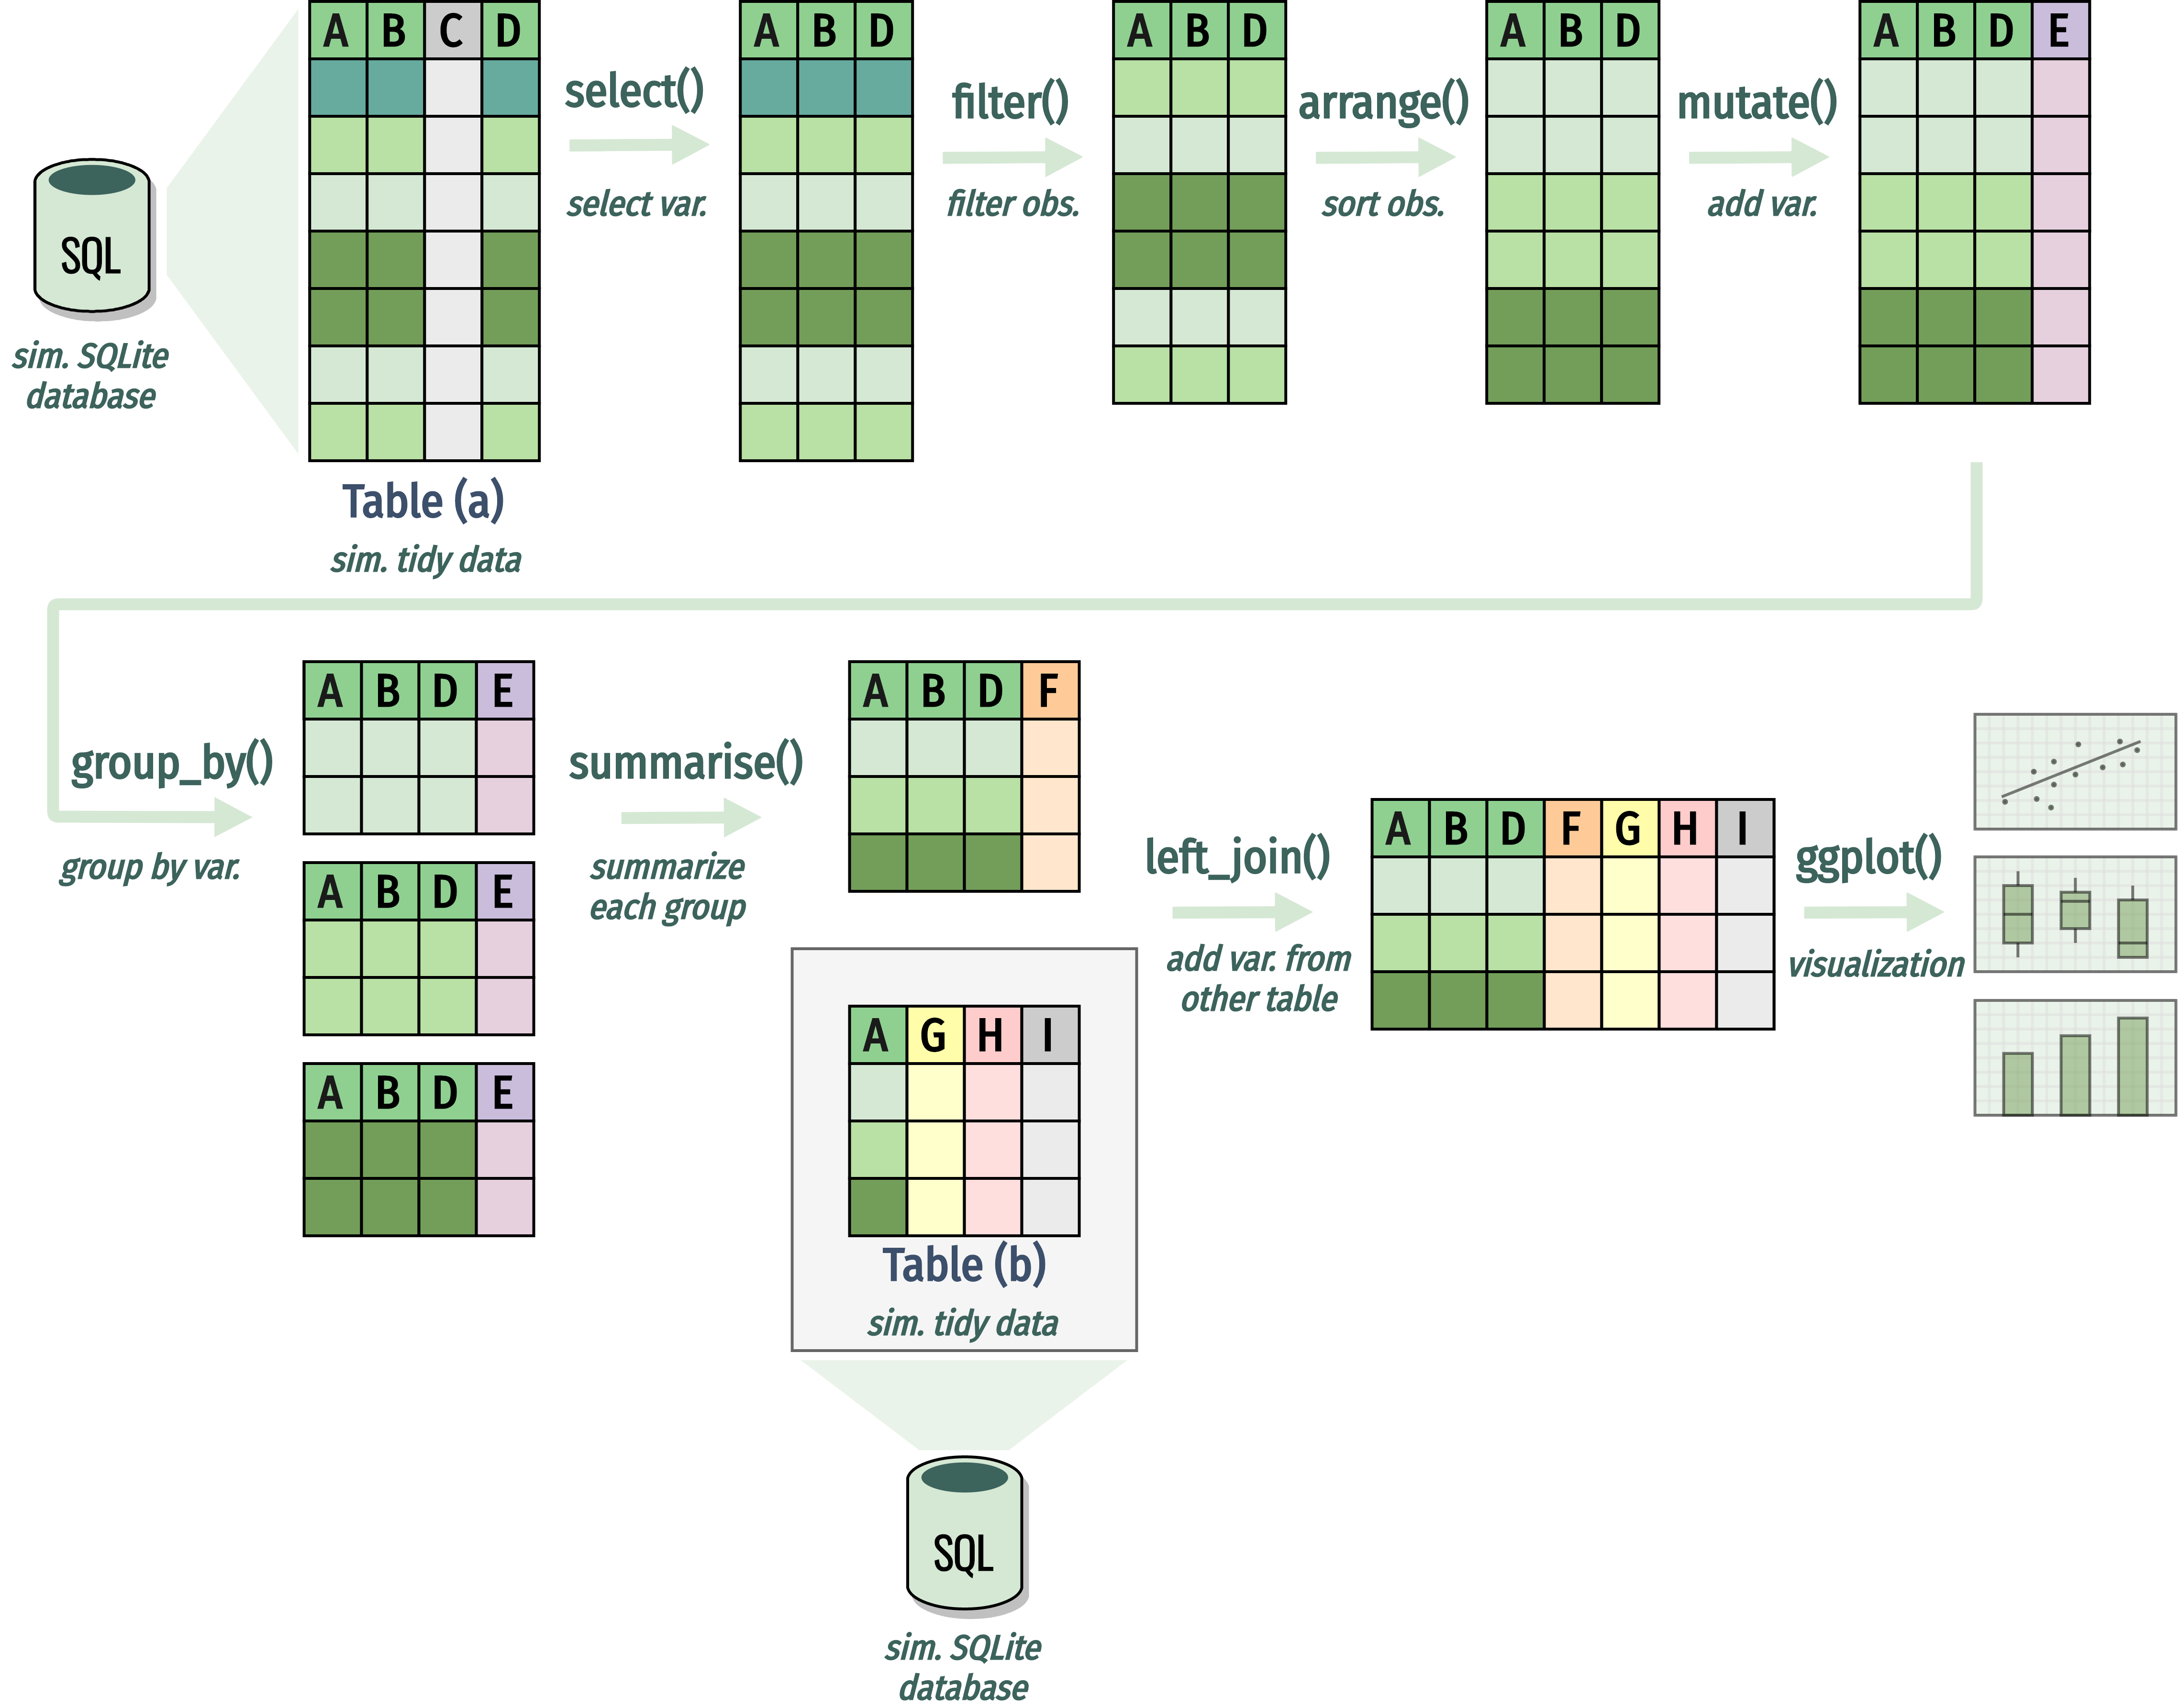
\includegraphics[width=0.7\linewidth]{/mnt/c/Users/hongy/Dropbox/github_repo/eplusr-paper/figures/data-exploration} \caption{Workflow overview of data exploration using BES output extracted by the tidy data interface}\label{fig:flow-data}
\end{figure}

Lines 51 -- 64 in Listing \ref{code:basic} shows how to use methods
\texttt{tabular\_data()} and \texttt{report\_data()} provided by the tidy data
interface to extract building area and building energy consumption, zone
metadata, and cooling and heating demands, with all formatted in a tidy
representation.
Note that instead of presenting the simulated date and time as strings,
the \texttt{report\_data()} adds a time-series column \texttt{datetime} in \texttt{POSIXct} based on
a derived year value using the algorithm described in Section
\ref{sec:eplusr-io}.
Moreover, the tidy data interface also provides a number of additional columns
shown in Fig. \ref{fig:tidy-extractor}, which makes it convenient and
straightforward to directly perform further data transformations.
Lines 71 -- 119 in Listing \ref{code:basic} demonstrate the benefits of the
tidy format in selecting columns using \texttt{select()}, subsetting rows using
\texttt{filter()}, sorting rows using \texttt{arrange()}, adding new variables using
\texttt{mutate()}, summarizing data using a combination of \texttt{group\_by()} and
\texttt{summarize()}, joining tables using \texttt{left\_join()}, and data visualization using
\texttt{ggplot()}.

Based on the building energy consumption data (line 54 in Listing
\ref{code:basic}) and the building area (line 51 in Listing
\ref{code:basic}), the monthly electricity consumption breakdown from various end-use
categories was calculated, and a stacked area chart was created (shown in Fig.
\ref{fig:eui}) (line 93 -- 107 in Listing
\ref{code:basic}). From Fig. \ref{fig:eui}, we can see that throughout the
year, most of the energy has been consumed by interior electric equipment,
followed by indoor lighting.
It indicates that ECMs which help to reduce the plug loads and lighting power
density (LPD) may have a promising potential in improving the overall energy
performance.
We will perform further investigations on this in Section \ref{sec:param}.

\begin{figure}[!htb]
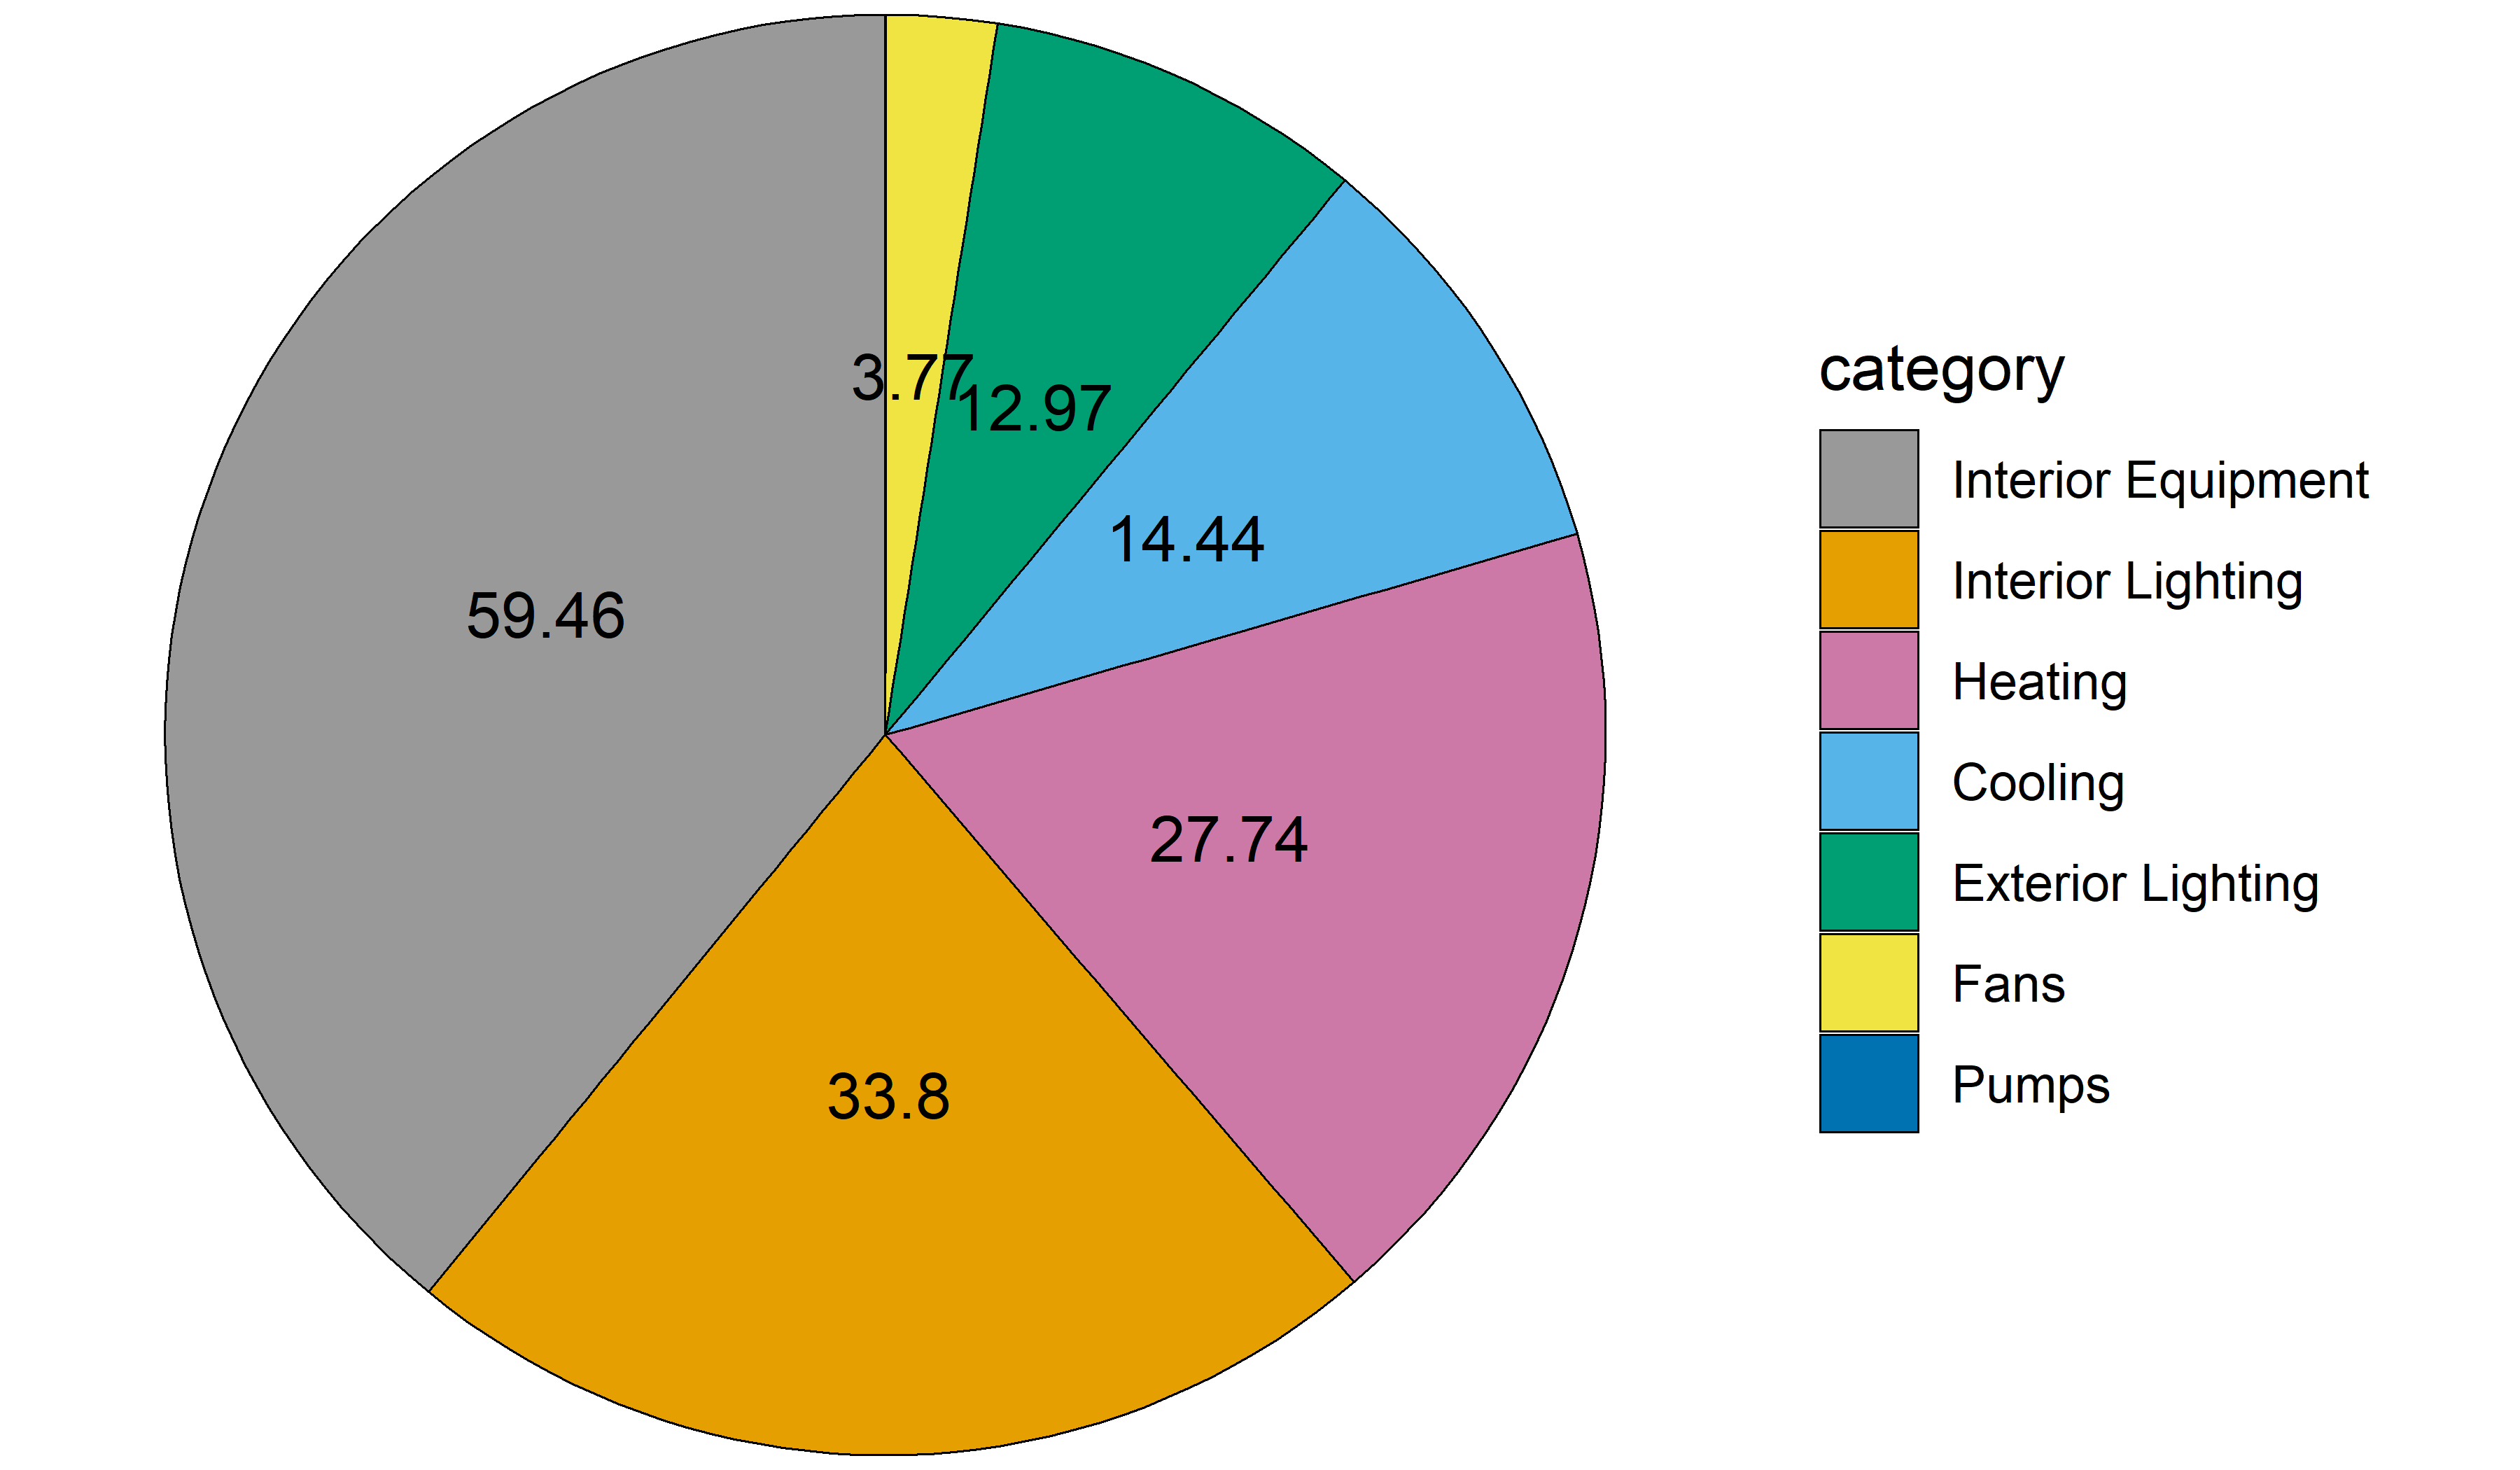
\includegraphics[width=0.5\linewidth]{/mnt/c/Users/hongy/Dropbox/github_repo/eplusr-paper/figures/eui} \caption{Monthly electricity consumption breakdown in $\mathrm{kWh}/\mathrm{m}^2$}\label{fig:eui}
\end{figure}

Fig. \ref{fig:signature} gives an energy signature diagram of outdoor air
temperature against electricity consumption a unit of \(\mathrm{GJ}\).
It is calculated based on the hourly outdoor air dry-bulb temperature
(line 60 -- 64 in Listing \ref{code:basic}) and hourly cooling and heating
electricity consumption extracted previously.
With the tidy format and additional time-series column, these two data fit well in the
data pipeline, making it straightforward and intuitive to perform data
transformation and visualization. In Fig. \ref{fig:signature}, we can
see that there is an obvious one tailed pattern for the cooling electricity usage.
There are large simultaneous heating and cooling operation hours, which may
indicate further improvements of control strategies needed to minimize reheat.
However, it is beyond the scope of this paper.

\begin{figure}[!htb]
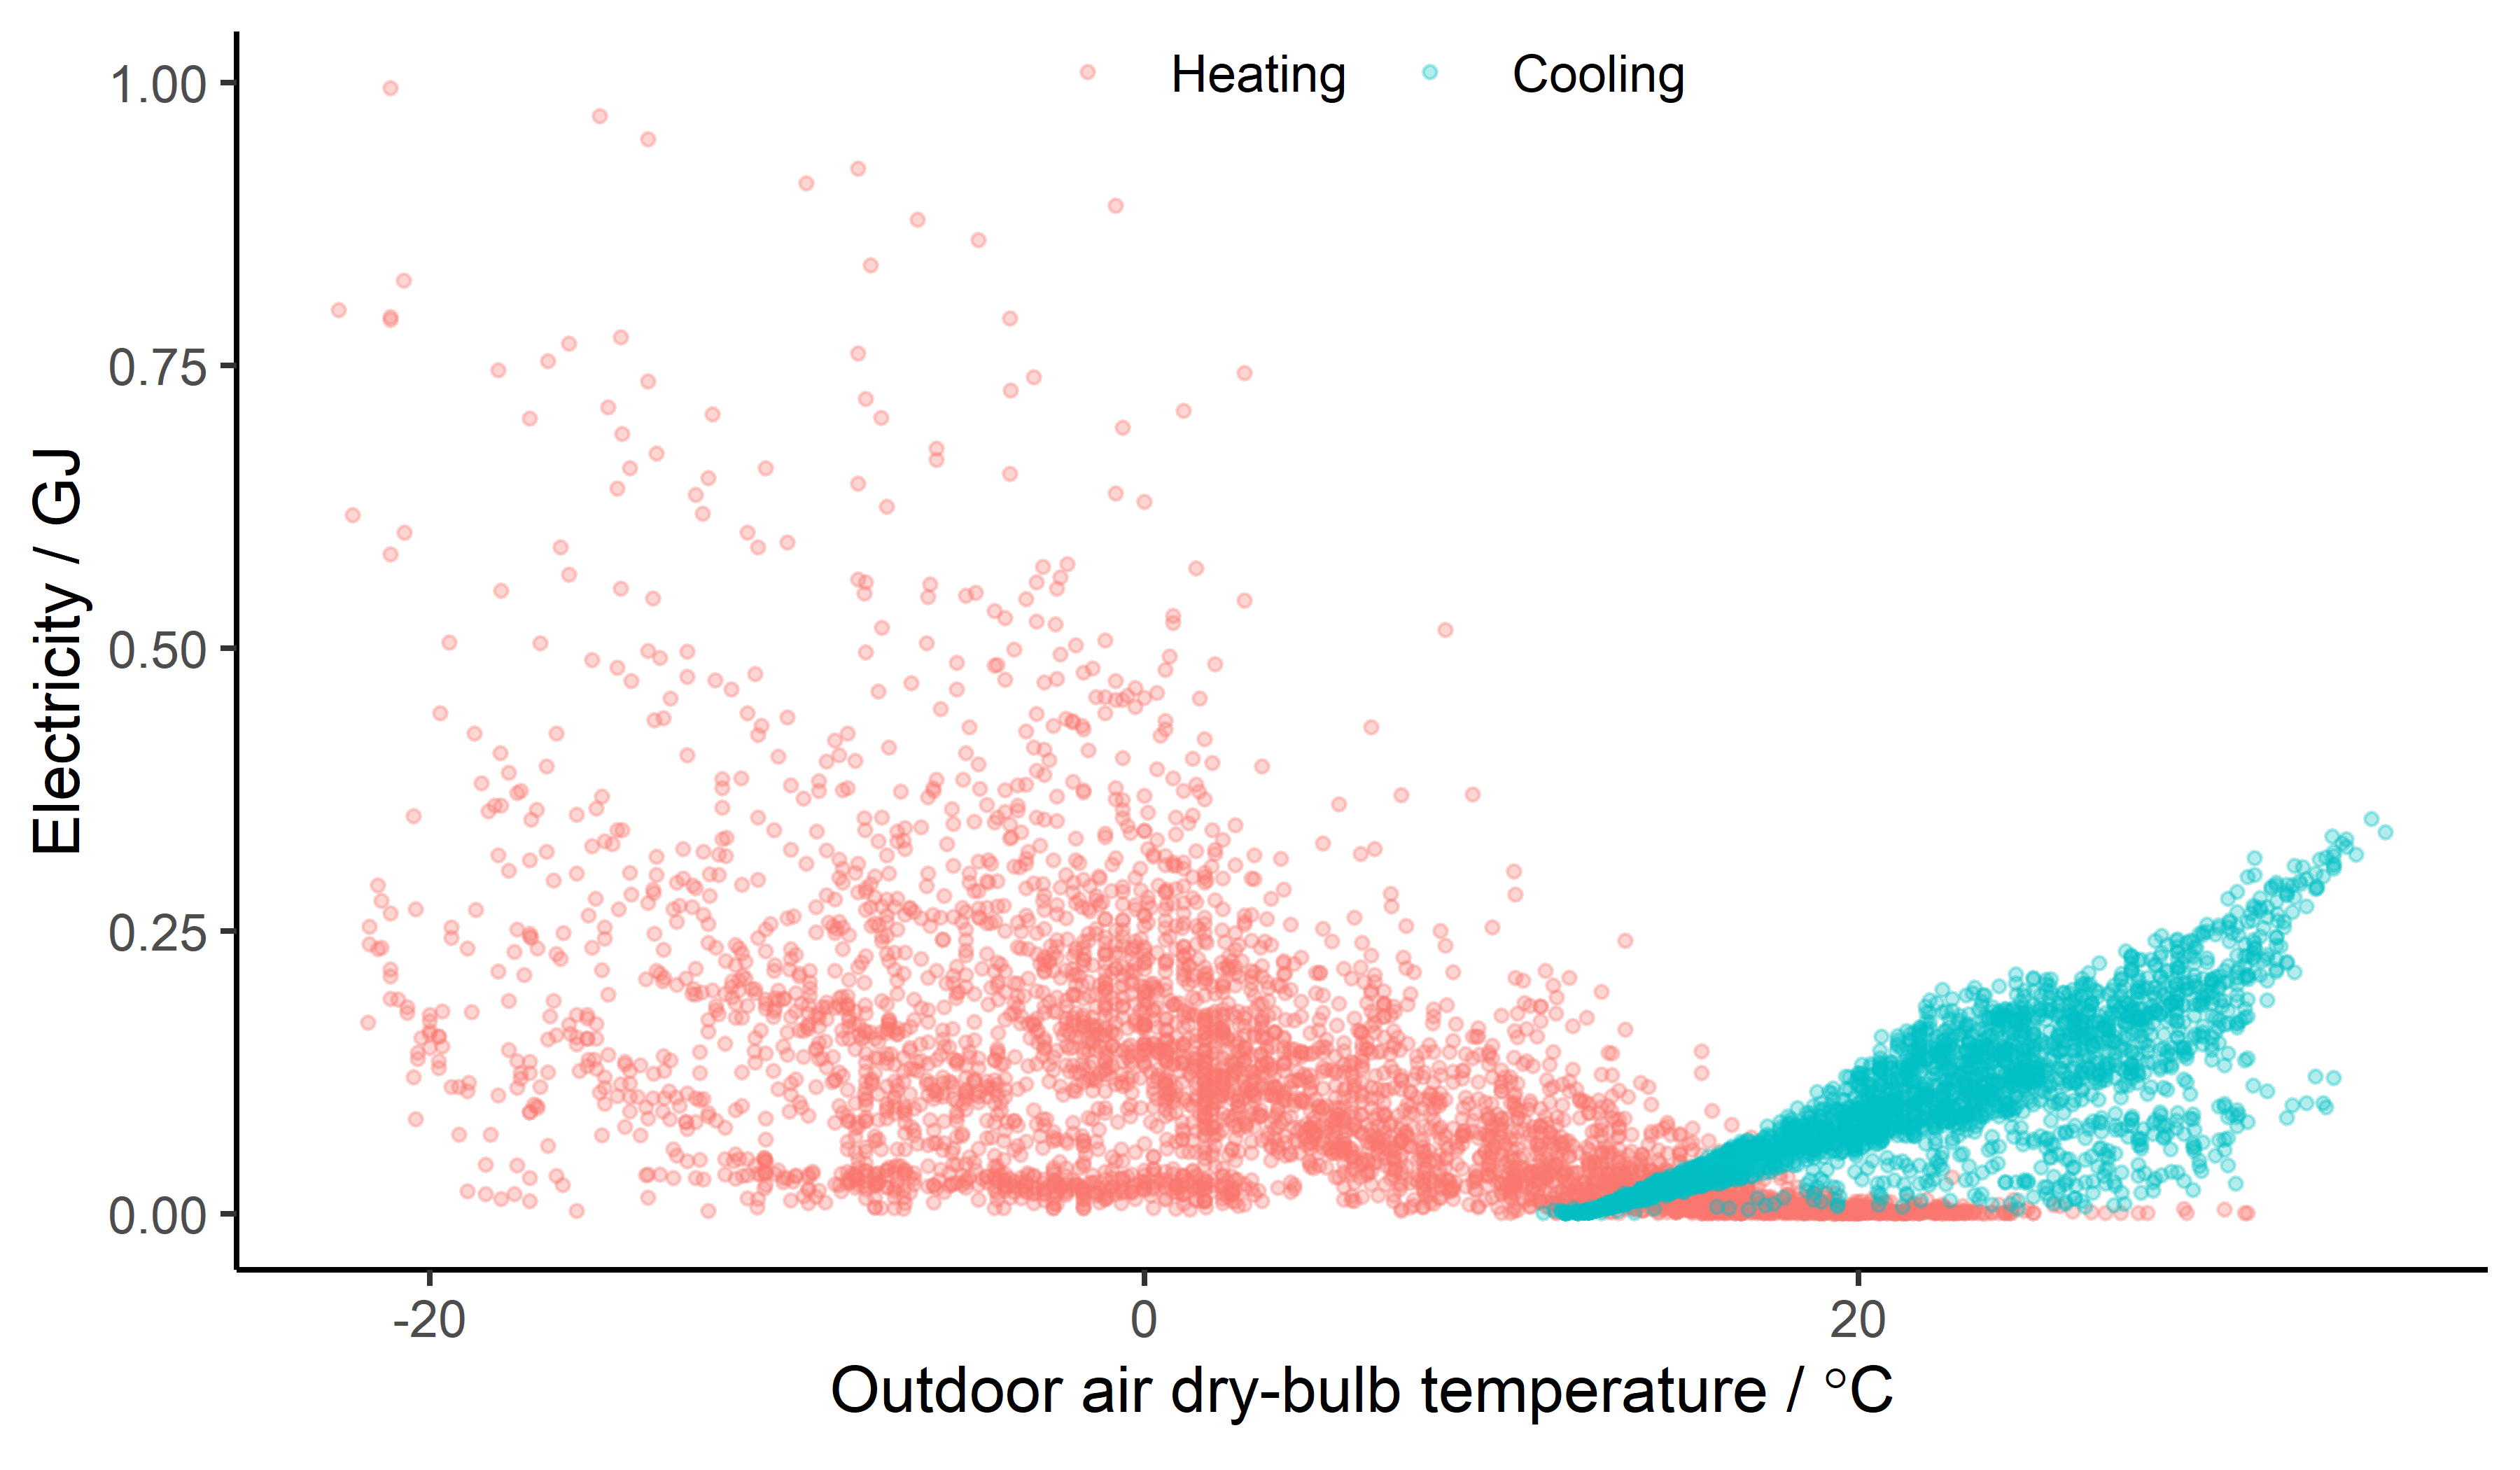
\includegraphics[width=0.5\linewidth]{/mnt/c/Users/hongy/Dropbox/github_repo/eplusr-paper/figures/mtr_temp} \caption{Energy signature diagram of outdoor temperature against electricity consumption}\label{fig:signature}
\end{figure}

\hypertarget{sec:param}{%
\subsection{Parametric simulation}\label{sec:param}}

This example demonstrates the process of performing parametric simulation
analyses using the proposed parametric prototype.
The main focuses are on showcasing the capabilities of (1) creating parametric
models by applying measures and (2) easing the comparative analysis by reusing
code snippets developed in data exploration process.

As shown in Fig. \ref{fig:eui}, the plug loads and interior lighting systems
consumed more than 60\% of total electricity.
In this example, we will investigate the energy-saving potentials of ECMs on
reducing the plug loads and LPD.
Fig. \ref{fig:flow-param} gives an overview of the workflow and Listing
\ref{code:param} shows the actual R code.

\begin{figure}[!htb]
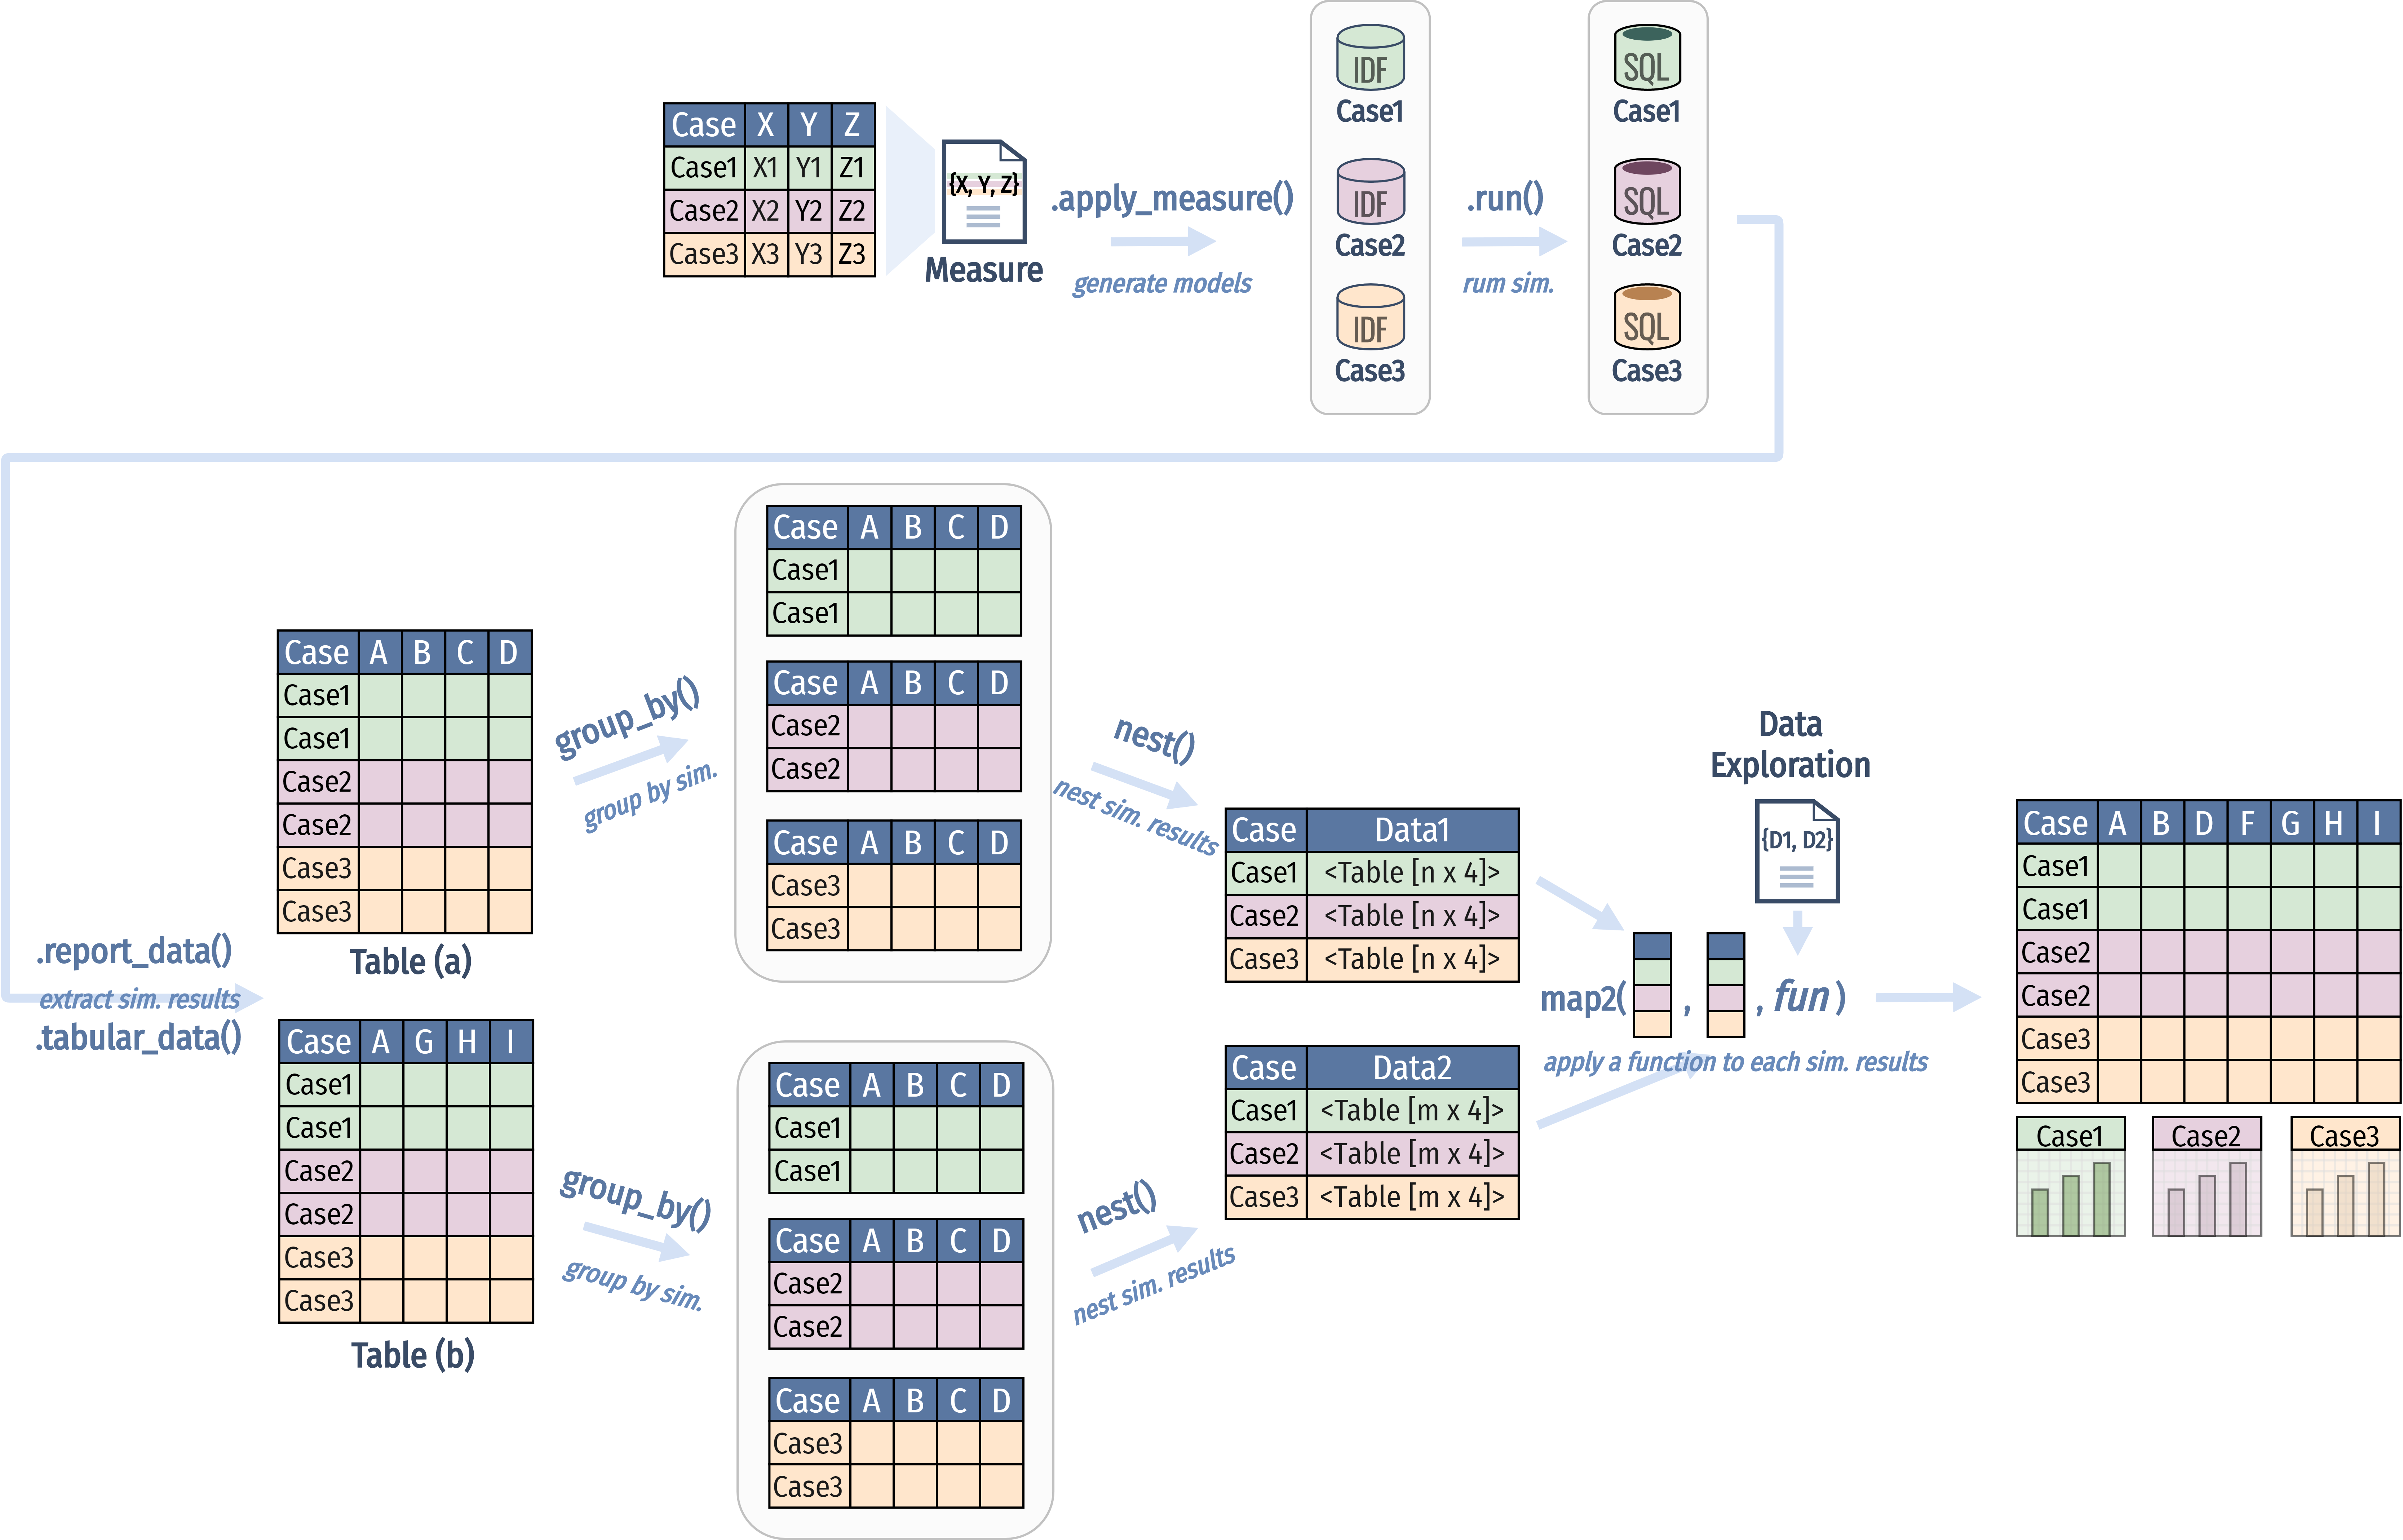
\includegraphics[width=1\linewidth]{/mnt/c/Users/hongy/Dropbox/github_repo/eplusr-paper/figures/parametric-simulation} \caption{Workflow overview of parametric simulation analysis using the proposed parametric prototype}\label{fig:flow-param}
\end{figure}

Measures are functions that describe how an energy model should be modified
based on input parameter values.
Lines 8 -- 18 in Listing \ref{code:param} shows a simple measure that modifies
the LPD.
The core code is line 14 that assigns all related fields in a whole class to
input values, taking advantage of the flexibly-scoped OOP model API.
Lines 20 -- 40 in Listing \ref{code:param} shows a measure that modifies the off-work
schedule values of plug loads by multiplying a specified reduction faction
value.
It demonstrates how objects in an energy model can be
translated into a table and how to use the modified table to alter
corresponding object values.

Different measures can be chained together and supplied to the
\texttt{apply\_measure()} method to create parametric models.
Each model will be tagged with a \emph{case} name as an identifier.
As demonstrated in lines 42 -- 57 in Listing \ref{code:param}, the
combined measure \texttt{ecm} is used to create six models with various combinations
of LPD and plug loads control strategies.

After calling the \texttt{run()} method to conduct parallel runs of simulations (line
60 in Listing \ref{code:param}), the tidy data interface can be used to
extract any simulation outputs of interest from the SQL database using
\texttt{report\_data()}, \texttt{tabular\_data()}, etc.
In this example, the building energy consumptions of all six
models are extracted using one line of code (line 67 in Listing \ref{code:param}).
The resulting data format is the same as that of a single simulation and is
equivalent to bind rows from six tables into one tidy table.
A \texttt{case} column is prepended using the names specified in line 56 in Listing
\ref{code:param}.
It works as an identifier to group the results by different parametric models
using \texttt{group\_by()} and \texttt{nest()} functions from the tidyverse package.
This data structure makes it effortless to perform comparative analyses by
taking the code snippets developed in data exploration for a single simulation
and applying them to each of the parametric simulations.
In this example, most of the EUI breakdown calculation code in Listing
\ref{code:basic} have been reused (lines 70 -- 77 in \ref{code:param}).
It also demonstrates how to use the \texttt{case} column to perform case filtering
(line 80 in Listing \ref{code:param}), table joins, and grouped summarization
(lines 84 -- 85 in Listing \ref{code:param}).

Fig. \ref{fig:savings} shows the energy savings of various lighting
technologies and plug loads control strategies, based on lines 82 -- 96 in
Listing \ref{code:param}. All technologies show overall energy savings to
various degrees. Using higher efficiency lightings shows promising
savings in both reducing the lighting electricity usage, with T5 and LED saving
34.9\%\% and 53.5\% respectively, and the corresponding overall energy savings for
T5 and LED are 7.5\% and 11.4\%. Strategies of turning off 40\% and an 80\%
unnecessary plug loads during off-work hours reduce 11.3\% and 22.6\% electricity
usage from interior equipment and improve the overall energy performance by
3.0\% and 5.8\%, respectively. Additional energy savings can be obtained when
incorporating LED with an 80\% reduction factor in off-work plug loads. However,
even the overall energy savings are positive for all cases, trend for
heating energy shows the opposite. This is due to the reason that all examined
technologies will reduce indoor heat gains which plays a positive role during
heating seasons.

\begin{figure}[!htb]
\includegraphics[width=0.6\linewidth]{/mnt/c/Users/hongy/Dropbox/github_repo/eplusr-paper/figures/savings} \caption{Energy savings of various lighting technologies and plug loads control strategies}\label{fig:savings}
\end{figure}

\hypertarget{multi-objective-optimization-using-genetic-algorithm}{%
\subsection{Multi-objective optimization using Genetic Algorithm}\label{multi-objective-optimization-using-genetic-algorithm}}

Automated optimization has become increasingly popular in BES research and
applications to efficiently search and identify optimal or near-optimal design
options meeting one or more key design performance objectives \citep{Attia2013a}.
Multi-objective optimization has also shown its potentials in building energy
simulation calibration \citep{Yang2015c}.
However, existing BES frameworks and applications for MOO often have
constraints in the number of optimization objectives and limited flexibility in
optimization parameter specifications.

The epluspar R package is an extension of the eplusr R package.
It implements a \texttt{GAOptimJob} class which is based on the parametric prototype
and the \emph{ecr} R package \citep{Bossek2017} for solving BES optimization problems
using the Genetic Algorithm (GA).
The \texttt{GAOptimJob} class leverages the proposed framework in terms of data
structure and parametric simulation management and is capable of defining any
number of arbitrary customized objective functions.
It implements flexible general-purpose GA interfaces to solve BES-based single-
or multi-objective optimization problems.
This example demonstrates how to use the \texttt{GAOptimJob} class to solve a MOO
problem, i.e.~reducing carbon emissions and discomfort hours of the medium
office reference building at the same time, by varying (1) indoor heating and
cooling setpoint temperatures, (2) window-to-wall ratio (WWR) and (3) exterior
wall insulation thickness.
Fig. \ref{fig:flow-ga} gives an overview of a typical GA-based MOO process
using the \texttt{GAOptimJob} class.
Listing \ref{code:moo} shows the actual R code.
The process shown in Fig. \ref{fig:flow-ga} can be divided into four main
parts:

\begin{enumerate}
\def\labelenumi{\arabic{enumi}.}
\tightlist
\item
  Specify optimization parameters
\item
  Create optimization objective functions
\item
  Set GA operators
\item
  Gather results and perform further analyses
\end{enumerate}

\begin{figure}[!htb]
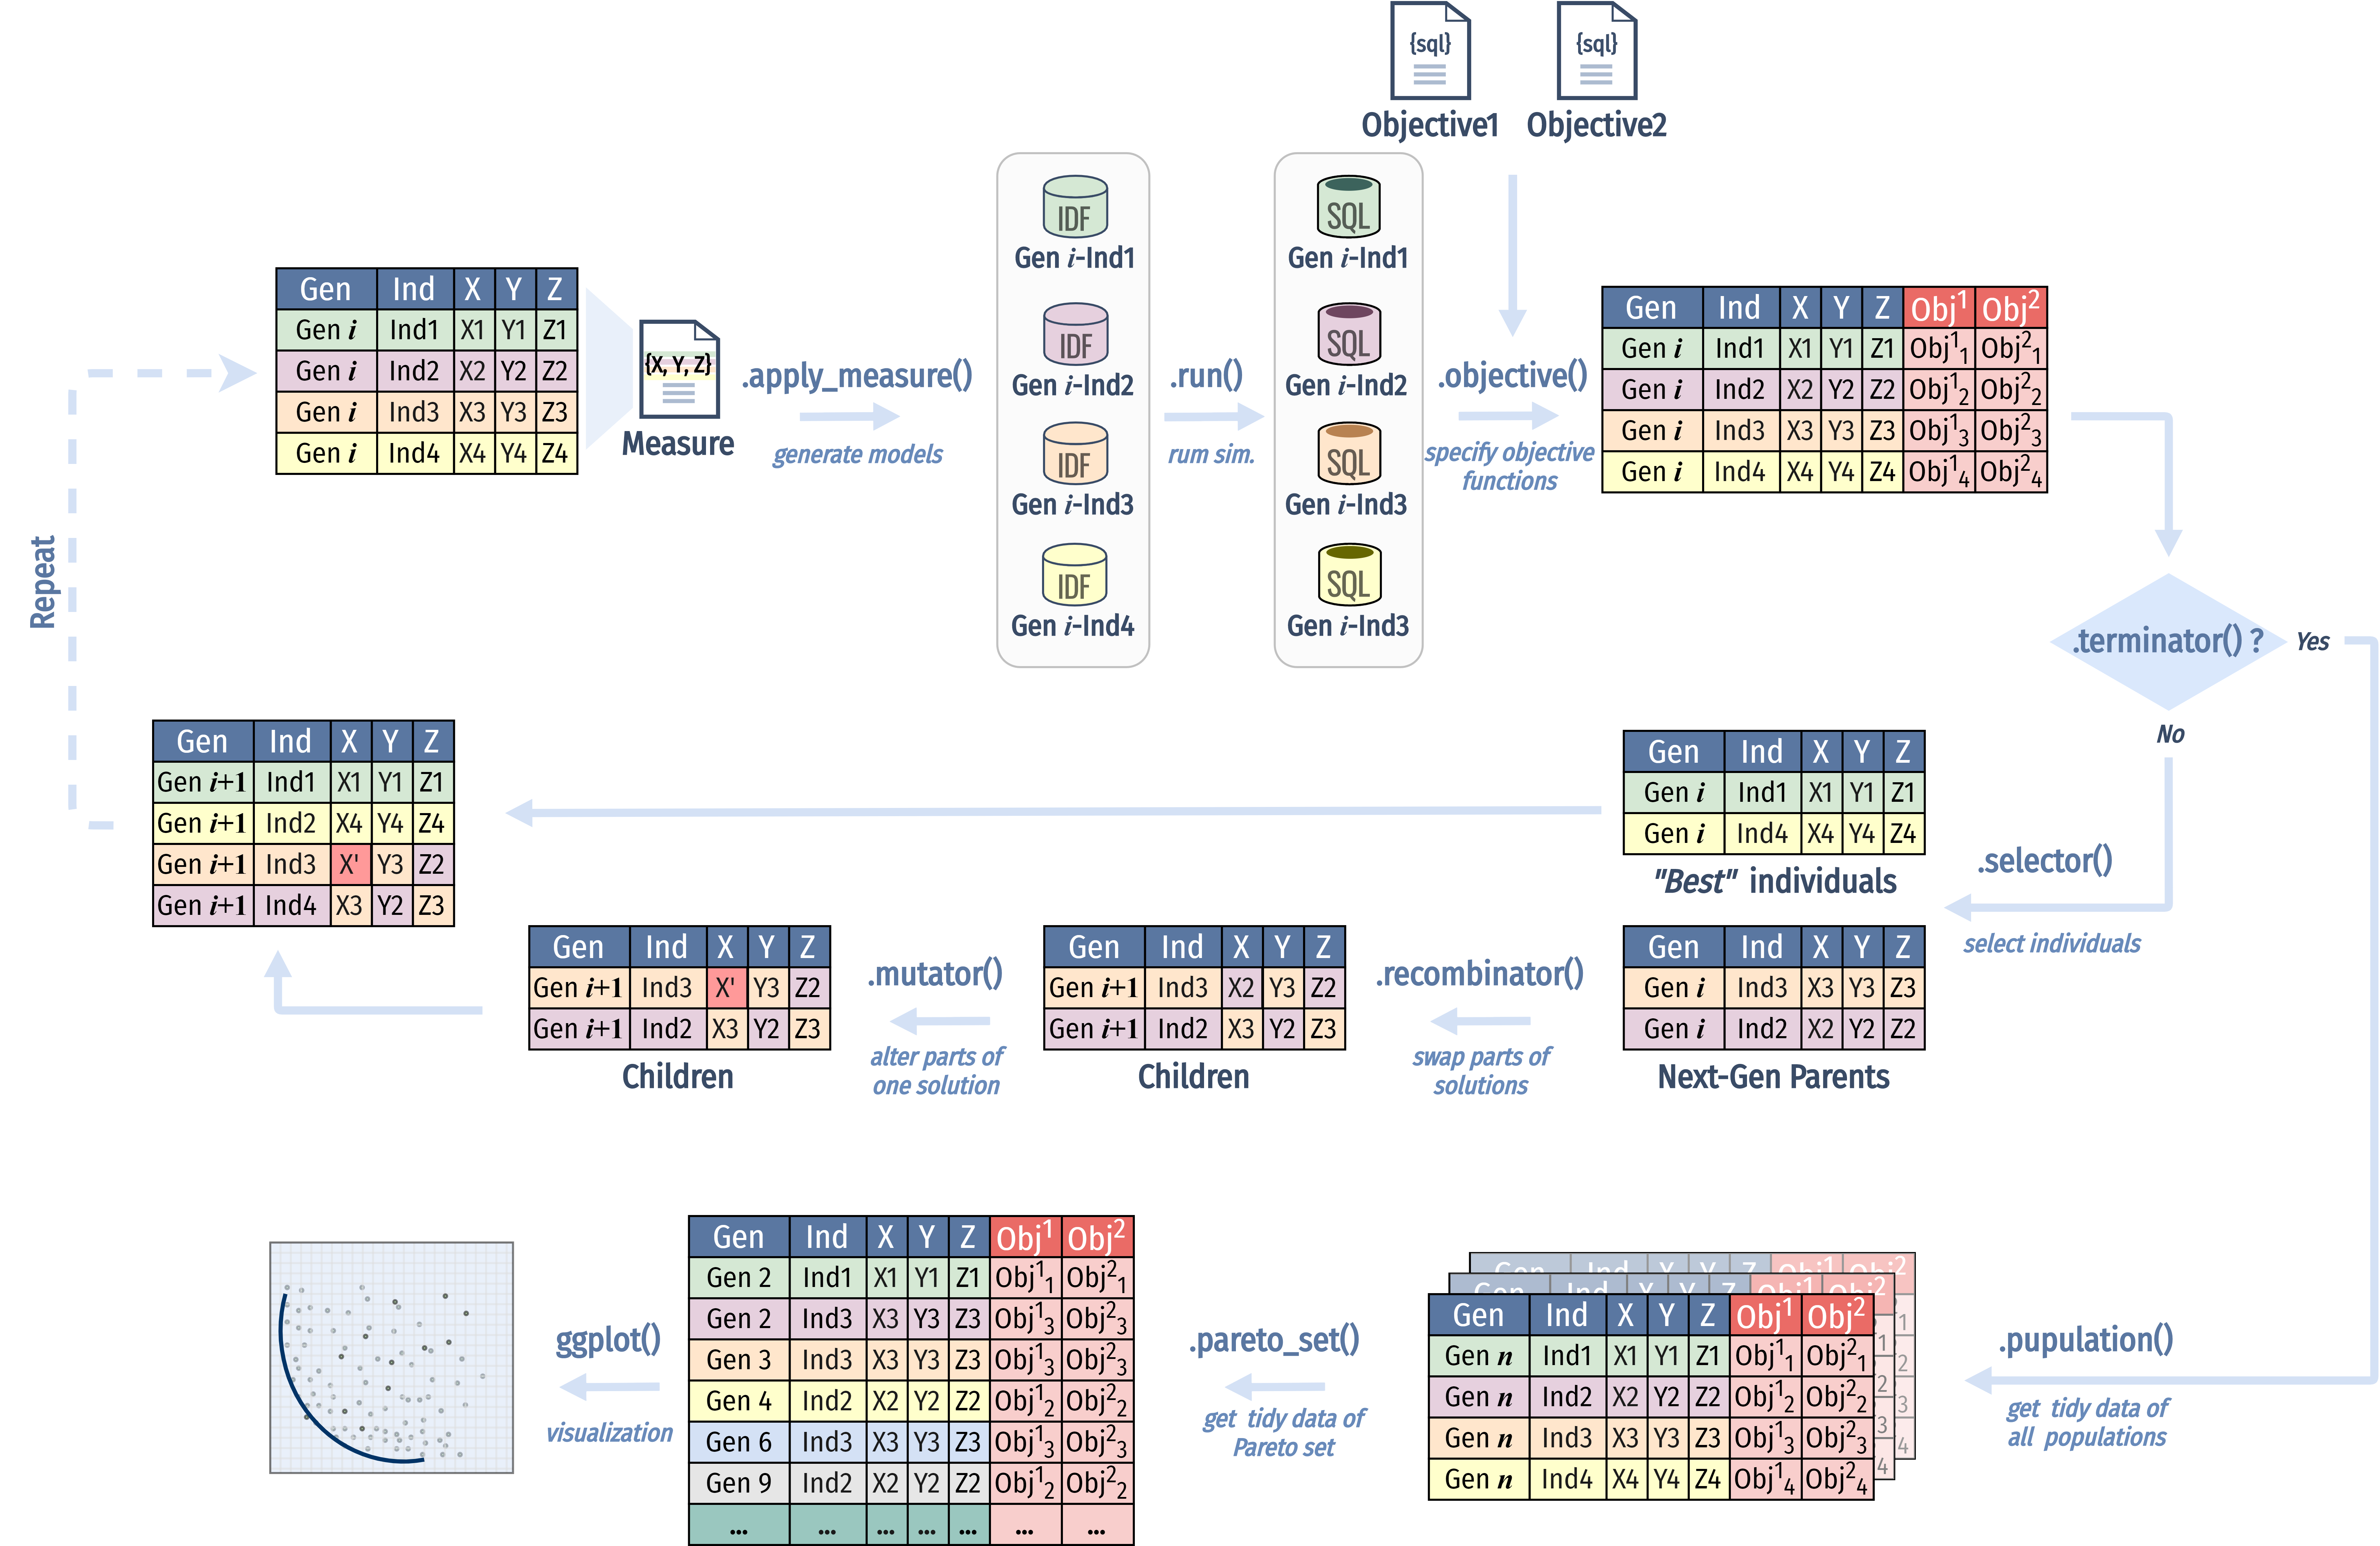
\includegraphics[width=1\linewidth]{/mnt/c/Users/hongy/Dropbox/github_repo/eplusr-paper/figures/MOO} \caption{Workflow overview of performing multi-objective optimization on an EnergyPlus model using the epluspar package that is based on the proposed parametric prototype}\label{fig:flow-ga}
\end{figure}

Built on top of the parametric prototype, \texttt{GAOptimJob} class provides a similar
interface for parametric model generation in the \texttt{apply\_measure()} method.
It can take the same measure functions to describe how optimization parameters
should be modified.
Lines 11 -- 62 in Listing \ref{code:moo} define three measure functions to
accept various design options in terms of (1) indoor heating and cooling set
point, (2) window-to-wall ratio (WWR) and (3) exterior wall insulation
thickness.
The actual optimization parameter values in each generation are automatically
calculated based on the GA operators and provided to \texttt{apply\_measure()} method
for parametric model generation.

\texttt{GAOptimJob} provides the flexibility to define objective functions of an
optimization problem using any results from the simulation outputs. The
\texttt{objective()} method takes objective definitions, evaluates them after
simulations, and extracts the fitness together with optimization parameter values
into a tidy table for post-processing using GA operators.
In this example, Lines 88 -- 95 in and lines 97--104 in Listing \ref{code:moo}
define functions to extract the annual total carbon emissions and discomfort
hours counted based on the Standard ASHRAE 55 -- 2004 from the standard reports
using tidy data interface.
The \texttt{objective()} method in Line 107 in Listing \ref{code:moo} takes these two
objective functions and tells the algorithm the minimization optimization
direction.

\texttt{GAOptimJob} class has three key genetic operators (methods): (1) \texttt{selector()}
(to select individuals to breed a new generation), (2) \texttt{mutator()} (to alter
parts of one solution randomly), and (3) \texttt{recombinator()} (also called
crossover, to swap parts of the solution with another), providing detailed
procedures and steps on how to generate children from parent solutions.
Lines 114 -- 118 in Listing \ref{code:moo} directly specify those three
operators with the default values that are tweaked to directly perform MOO
using the Non-Dominated Sorting Genetic Algorithm (NSGA-II).
The \texttt{terminator()} method is used to specify conditions to terminate the
computation.
In this example, we set it to stop when one hundred generations have been
evaluated.

With all objectives, parameters, and operators specified, the optimization will
start with the \texttt{run()} method.
In this example, we have 20 individuals per generation, resulting in a
total of 2000 annual energy simulations.
Once one of the conditions specified in \texttt{terminator()} is met, all populations
and Pareto set can be extracted into two tidy tables for further analyses,
using the \texttt{population()} and \texttt{pareto\_set()} method (Lines 130 and 133 in Listing
\ref{code:moo}).
Fig. \ref{fig:pareto} shows the Pareto front of discomfort hours and total
carbon emissions generated using lines 135 -- 143 in Listing \ref{code:moo}.
The final Pareto font contained 20 unique solutions.

\begin{figure}[!htb]
\includegraphics[width=0.4\linewidth]{/mnt/c/Users/hongy/Dropbox/github_repo/eplusr-paper/figures/pareto} \caption{Pareto front of discomfort hours and carbon emissions}\label{fig:pareto}
\end{figure}

Fig. \ref{fig:parallel} shows the parallel coordinates charts of the Pareto
set. The carbon emissions have seen a significant reduction from the original
value of 290ton. However, there were 10 out of 20 solutions in the Pareto set
that performed worse in terms of providing a satisfactory indoor thermal
environment. One possible solution to avoid this is to add a constraint when
evaluating the fitness of the \texttt{discomfort\_hours} objective, making sure all
solutions that have larger discomfort hours should be abandoned.

\begin{figure}[!htb]
\includegraphics[width=0.7\linewidth]{/mnt/c/Users/hongy/Dropbox/github_repo/eplusr-paper/figures/parallel} \caption{Parallel coordinates chart of the Pareto set}\label{fig:parallel}
\end{figure}

\hypertarget{bayesian-calibration}{%
\subsection{Bayesian calibration}\label{bayesian-calibration}}

Model calibration is an essential process to achieve greater confidence in BES
results. In recent years there has been an increasing application of Bayesian
approaches for BES calibration \citep{Chong2017, Tian2016Identifying, Yi2019Parameter}. Bayesian calibration is carried
out following the statistical formulation proposed by Kennedy and O'Hagan
\citep{Chong2018}. This example demonstrates the model calibration workflow
using the epluspar R package. The epluspar R package implements the Bayesian
calibration algorithm proposed by Chong \citep{Chong2017} and guidelines proposed by
Chong and Menberg \citep{Chong2018}, and encapsulates them into the \texttt{BayesCalibJob}
class.
The \texttt{BayesCalibJob} class inherits from the parametric prototype and thus can
leverage all the parametric simulation management capabilities.

Fig. \ref{fig:flow-bc} gives an overview of a typical workflow of Bayesian
calibration using the \texttt{BayesCalibJob} class in the epluspar package.
Specifically, Listing \ref{code:bc} shows the workflow of calibrating one VAV
fan total efficiency in the medium office reference model using observed fan
air flow rate and electrical power.

\begin{figure}[!htb]
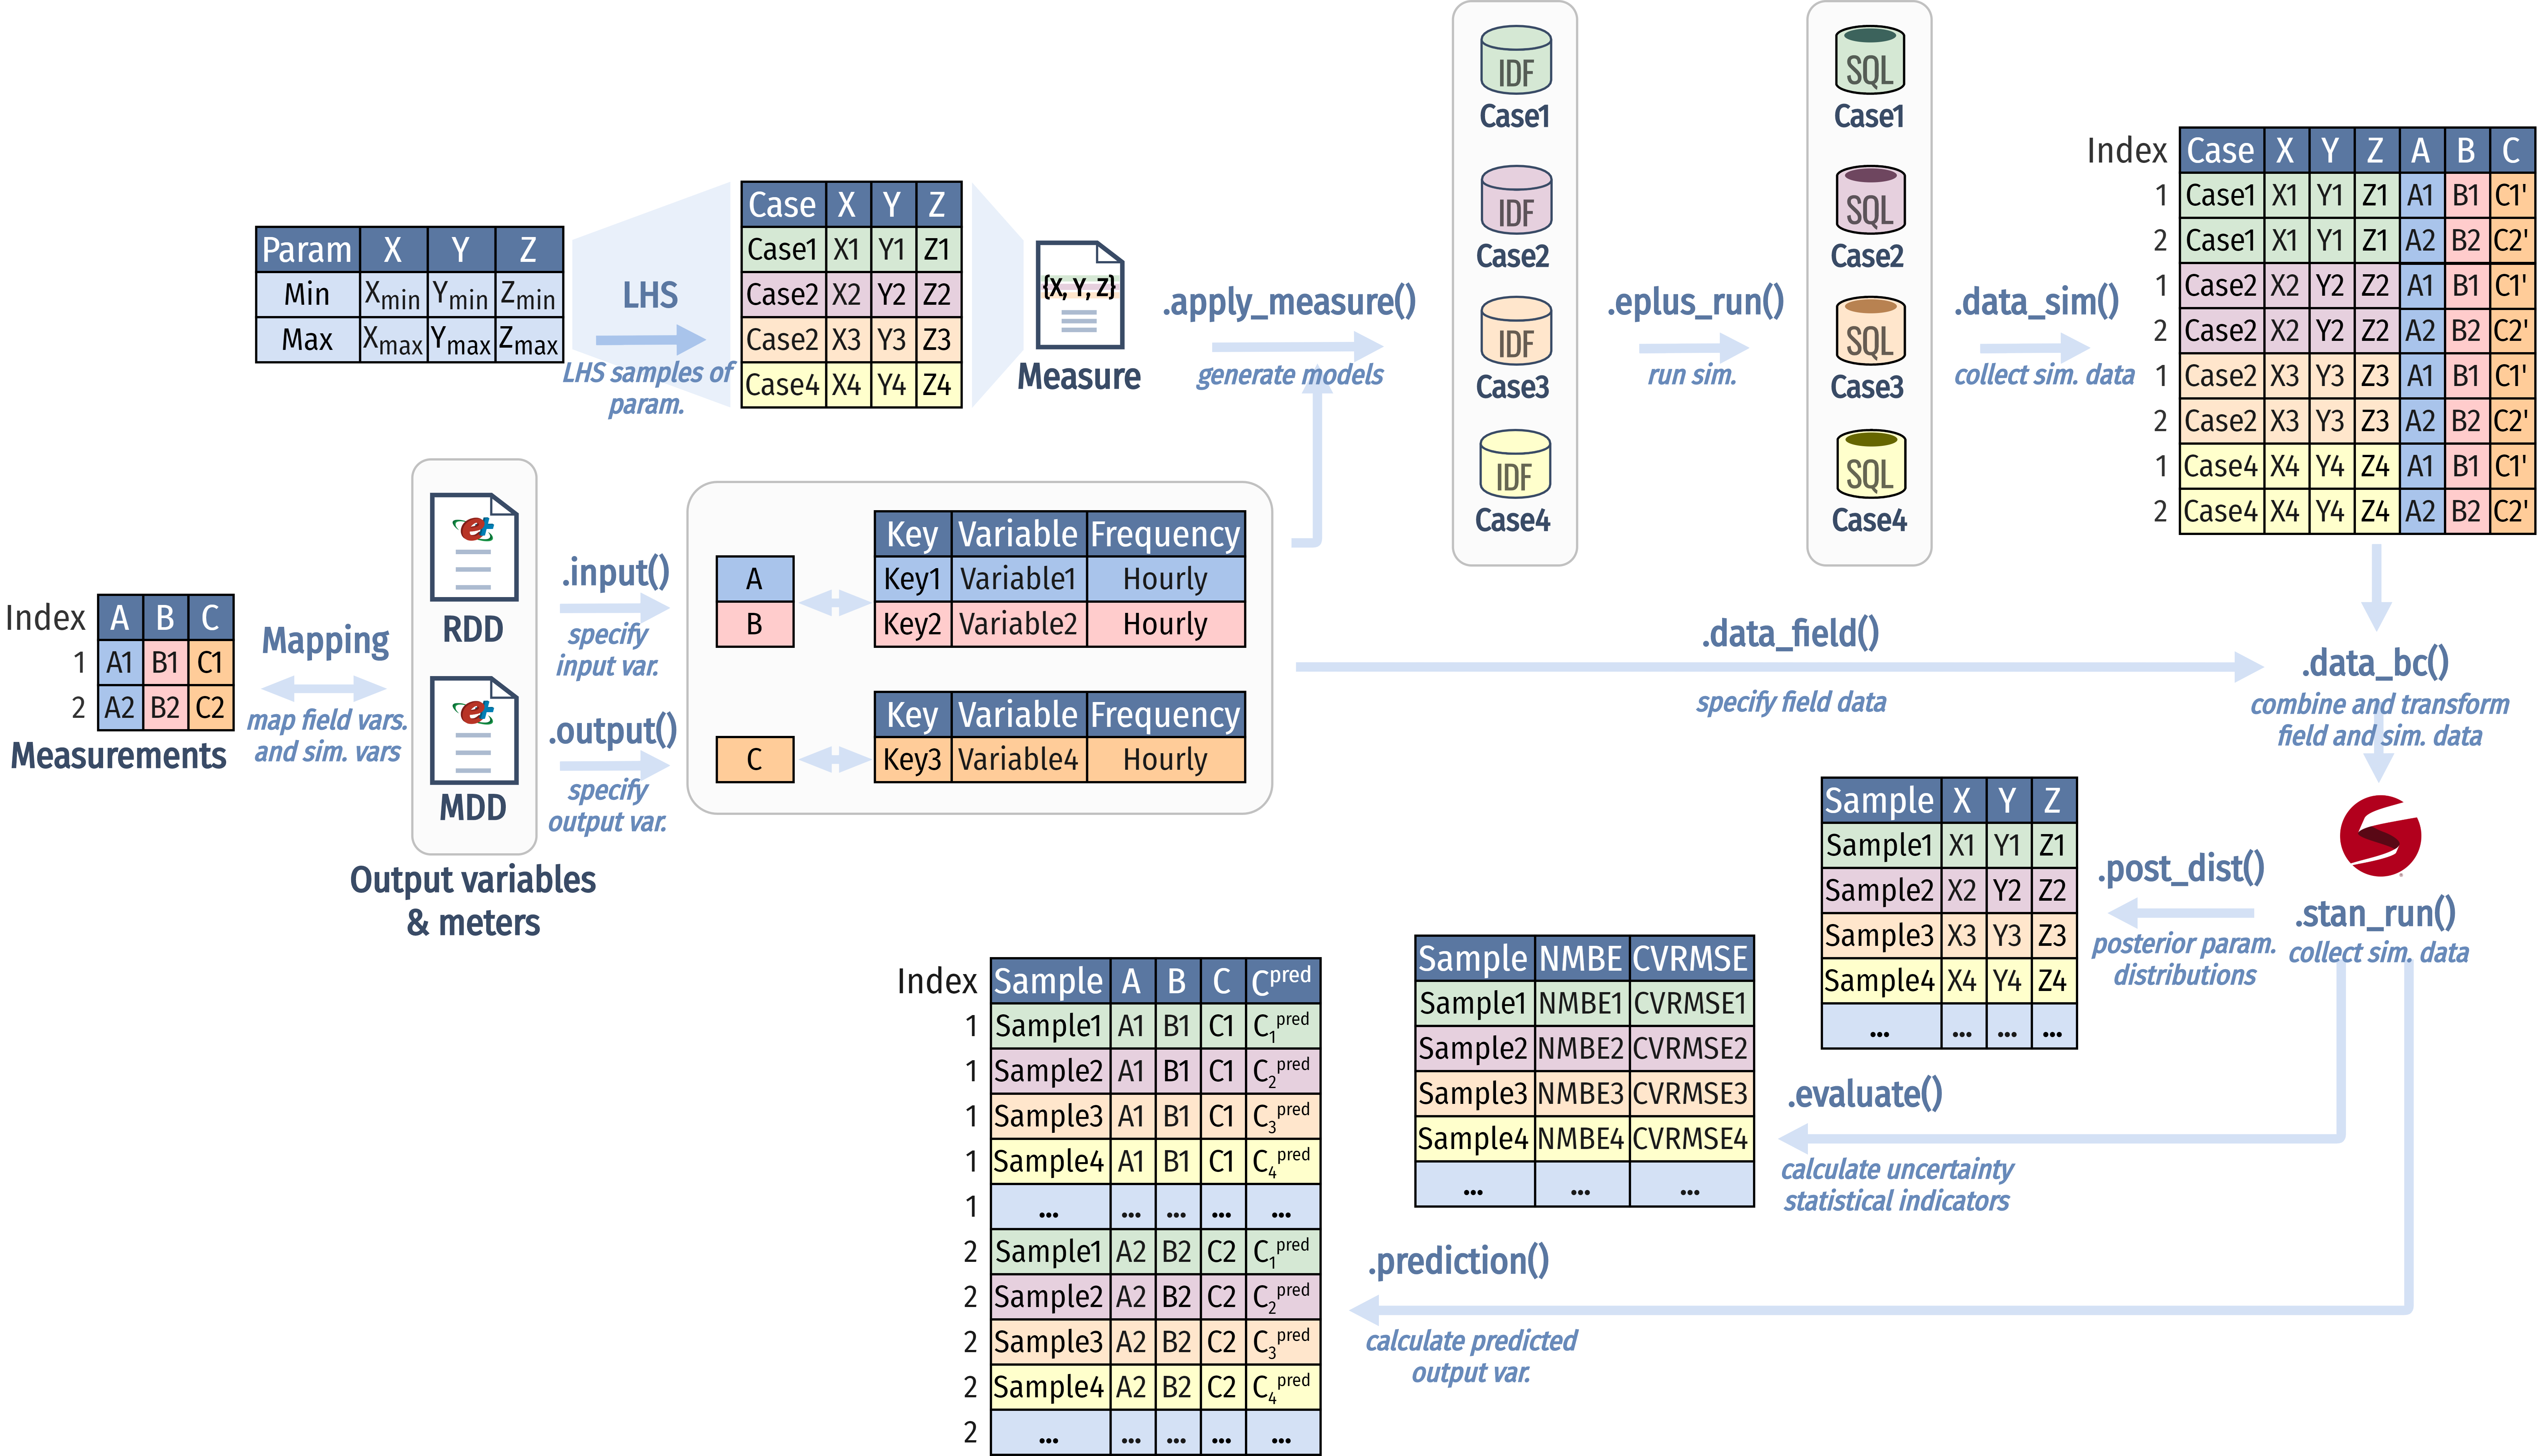
\includegraphics[width=1\linewidth]{/mnt/c/Users/hongy/Dropbox/github_repo/eplusr-paper/figures/BC} \caption{Workflow overview of performing Bayesian calibration on an EnergyPlus model using the epluspar package that is based on the proposed parametric prototype}\label{fig:flow-bc}
\end{figure}

The initial step for a Bayesian calibration is to collect data for observable
input and output.
In this example, since the reference model represents a virtual building with
no measured data, we created some synthetic data for the examined period of July
1st to July 3rd using simulations (lines 1 -- 27 in Listing \ref{code:bc}).
Also, the TMY3 weather data was used, instead of the Actual Meteorological Year
(AMY) weather data.
In real practice, the actual measurable variables may not be directly
representable in EnergyPlus.
In this case, an essential mapping process has to be performed to transform
measured variables into EnergyPlus output variables (listed in RDD) and meters
(listed in MDD), and connect the transformed measured values with the model
using schedule files or other techniques.
The next step is to specify the observable input and output variables for the
calibration using the \texttt{input()} and \texttt{output()} methods in \texttt{BayesCalibJob} class
(lines 30 -- 40 in Listing \ref{code:bc}).

Following the Bayesian calibration guidelines described in \citep{Chong2018},
the epluspar R package also introduces a \texttt{SensitivityJob} class based on the
parametric prototype to perform calibration parameter screening with the Morris
method.
In \texttt{BayesCalibJob} class, the calibration parameters, together with the number
of EnergyPlus simulations, can be described using either the \texttt{param()} method
(lines 42 -- 46 in Listing \ref{code:bc}) or the \texttt{apply\_measure()} method.
Each calibration parameter should be given a lower and upper bound value.
Once the calibration parameters are given, the Latin Hypercube Sampling (LHS)
algorithm will be used to generate parameter sample values based on the lower
and upper bound and the simulation number (lines 48 -- 49 in Listing
\ref{code:bc}).
The benefit of LHS is that it will try to cover as much as possible in the
multi-dimensional space of the calibration parameters.

After completing all simulations using the \texttt{eplus\_run()} method (lines 51 -- 52
in Listing \ref{code:bc}), the \texttt{data\_sim()} method gathers all simulated data of
calibration input and output variables and aggregates the data into the same
time frequency as the actual measured data (lines 54 -- 55 in Listing
\ref{code:bc}).
Method \texttt{data\_bc()} will combine measured data and simulated data, and transform
them into a list with the proper format for the Bayesian calibration algorithm
(lines 60 -- 61 in Listing \ref{code:bc}) written in probabilistic programming
language Stan.
With all data required specified, the \texttt{stan\_run()} method is used to call the
Stan program (lines 63 -- 64 in Listing \ref{code:bc}).
Once completed, the posterior distributions of calibration parameters and
predicted output variable values can be retrieved using method \texttt{post\_dist()}
and \texttt{prediction()}, respectively (lines 66 -- 70 in Listing \ref{code:bc}).
The uncertainty statistical indicators, including Normalized Mean Biased
Error (NMBE) and Coefficient of Variation of the Root Mean Squared Error
(CVRMSE) can be retrieved using the \texttt{evaluate()} method (lines 72 -- 73 in Listing \ref{code:bc}).
Each method returns a tidy table that is well fit for the tidyverse data
pipeline for data transformation and visualization.

Fig. \ref{fig:dist-post} gives a density plot showing the posterior
distributions of calibrated fan total efficiency, created using lines 75 -- 80
in Listing \ref{code:bc}. The mean value of the posterior distribution was
0.60, which is quite close to the actual value of 0.59 specified in the
original model. Fig. \ref{fig:uncertainties} gives a box plot showing the
distribution of CVRMSE and NMBE per Markov Chain Monte Carlo (MCMC) sampling,
created using lines 82 -- 86 in Listing \ref{code:bc}. The mean NMBE value was
quite close to zero, and the average CVRMSE is around 3.0\%. Both values met the
thresholds of CVRMSE \(\leq\) 15\% and NMBE \(\leq\) 5\% set by ASHRAE \citep{ASHRAE2014}.
The satisfactory results are expected since we use synthetic data. However,
the overall workflow shown in this example can be applied to Bayesian
calibration on building energy models with real measured data.

\begin{figure}[!htb]
\includegraphics[width=0.4\linewidth]{/mnt/c/Users/hongy/Dropbox/github_repo/eplusr-paper/figures/dist-post} \caption{Posterior distribution of fan total efficiency}\label{fig:dist-post}
\end{figure}

\begin{figure}[!htb]
\includegraphics[width=0.4\linewidth]{/mnt/c/Users/hongy/Dropbox/github_repo/eplusr-paper/figures/uncertainties} \caption{Distribution of CVRMSE and NMBE per MCMC sample}\label{fig:uncertainties}
\end{figure}

\hypertarget{discussion}{%
\section{Discussion}\label{discussion}}

The four example applications have further confirmed the value of structured
BES inputs and outputs in providing seamless integration between BES and
data-driven analytics. The parametric manager also provides new possibilities
to leverage existing advanced statistical modeling and machine learning tools
with the consistent data structure in large-scale parametric simulations.
Also, the parametric manager provides new possibilities to leverage existing
advanced statistical modeling and machine learning tools with consistent data
structure in large-scale of parametric simulations.
Currently, more and more BES tools and interfaces adopt Docker and
containerization to provide configurable technology stacks and take advantage
of high-performance computing (HPC) and the merging cloud-based resources
\citep{Ball2020open, Karaguzel2019Open}.
To the authors' knowledge, the proposed framework is the first one
that focuses on seamless integration between BES and data-driven analytics, and
BES reproducibility.
The data-centric design philosophy and open-sourced nature of the proposed framework can help advocate data-driven BES research with better credibility and transparency

However, the framework presented has some limitations that should be acknowledged.
The main limitation of the proposed framework lies in its R-oriented workflows,
which currently may not be widely adopted in industry fields. Prospective users
of the framework who do not know R must spend time learning how to use it. This
drawback may be compensated by the growing user community. Since the eplusr
framework is mainly focused on modifying existing BES models, instead of
creating new ones from scratch, currently it has limited capacities to perform
sophisticated geometry transformation, including surface matching and rotation.
Operations such as creating or replacing one whole HVAC system may also be
time-consuming processes.

\hypertarget{conclusion}{%
\section{Conclusion}\label{conclusion}}

Building energy simulation (BES) has been widely adopted for the investigation of
environmental and energy performance for different design and retrofit
alternatives. The absence of seamless integration of BES and data-centric
analysis raises problems in both the productivity and also the credibility of
BES studies. This paper proposed a holistic framework called `eplusr' to
bridge the gap between the building energy simulation and data science domains.

Eplusr differs from existing frameworks by its data-centric design philosophy.
It provides a tidy data interface for BES that matches the semantics of the
simulation results with the data representation. The tidy data interface
provides the possibility to query BES outputs with various types of
specifications, which makes it easy and straightforward to extract simulation
results from any time period and for any variables in a consistent manner. The
tidy-formatted results can be easily fed to various data-centric analytics
using existing tools in R.

The parametric prototype developed in this framework provides a set of
abstractions to ease the process of parametric model generation, design
alternative evaluation, and large parametric simulation management. It is
capable of defining various analyses using any algorithms available in R. The
flexibility and extensibility of the parametric simulation prototype in this
framework are demonstrated by its easy adoption to perform multi-objective
optimization and Bayesian calibration.

The need for reproducibility in BEM is growing significantly, together with the
ongoing trend of the increasing complexity of BEM projects. The eplusr framework
provides a solution by developing a portable and reusable BES
computational environment based on Docker containerization, encapsulating the
toolchains for statistical computing, building energy modeling, data analytics,
and literate programming. The open-source nature of the proposed framework will
advocate the BES domain to embrace the tools essential for maintaining a
reproducible workflow.

\hypertarget{supplementary-materials}{%
\section*{Supplementary materials}\label{supplementary-materials}}
\addcontentsline{toc}{section}{Supplementary materials}

The supplementary files include code and datasets used in this article. More
is available at https://github.com/ideas-lab-nus/eplusr-paper.

\hypertarget{acknowledgements}{%
\section*{Acknowledgements}\label{acknowledgements}}
\addcontentsline{toc}{section}{Acknowledgements}

This research was funded by the Republic of Singapore's National Research
Foundation through a grant to the Berkeley Education Alliance for Research in
Singapore (BEARS) for the Singapore-Berkeley Building Efficiency and
Sustainability in the Tropics (SinBerBEST) Program. BEARS has been established
by the University of California, Berkeley as a center for intellectual
excellence in research and education in Singapore.

\hypertarget{references}{%
\section*{References}\label{references}}
\addcontentsline{toc}{section}{References}

\hypertarget{refs}{}

\clearpage

\begin{appendices}

\renewcommand{\thesection}{\Alph{section}.}

\hypertarget{code-for-data-exploration}{%
\section{Code for data exploration}\label{code-for-data-exploration}}

\begin{Shaded}

\begin{Shaded}
\begin{Highlighting}[]
\CommentTok{# install packages}
\KeywordTok{install.packages}\NormalTok{(}\KeywordTok{c}\NormalTok{(}\StringTok{"eplusr"}\NormalTok{, }\StringTok{"tidyverse"}\NormalTok{))}

\CommentTok{# load package}
\KeywordTok{library}\NormalTok{(eplusr)}
\KeywordTok{library}\NormalTok{(tidyverse) }\CommentTok{# for data-driven analytics}

\CommentTok{# get EnergyPlus v9.1 installation directory}
\NormalTok{dir <-}\StringTok{ }\KeywordTok{eplus_config}\NormalTok{(}\FloatTok{9.1}\NormalTok{)}\OperatorTok{$}\NormalTok{dir}

\CommentTok{# use example model and weather file distributed with EnergyPlus v9.1}
\NormalTok{path_model <-}\StringTok{ }\KeywordTok{file.path}\NormalTok{(dir, }\StringTok{"ExampleFiles/RefBldgMediumOfficeNew2004_Chicago.idf"}\NormalTok{)}
\NormalTok{path_weather <-}\StringTok{ }\KeywordTok{file.path}\NormalTok{(dir, }\StringTok{"WeatherData/USA_IL_Chicago-OHare.Intl.AP.725300_TMY3.epw"}\NormalTok{)}

\CommentTok{# read model}
\NormalTok{idf <-}\StringTok{ }\KeywordTok{read_idf}\NormalTok{(path_model)}

\CommentTok{#############}
\CommentTok{# Model API #}
\CommentTok{#############}

\CommentTok{# make sure weather file input is respected}
\NormalTok{idf}\OperatorTok{$}\NormalTok{SimulationControl}\OperatorTok{$}\NormalTok{Run_Simulation_for_Weather_File_Run_Periods <-}\StringTok{ "Yes"}

\CommentTok{# make sure energy consumption is presented in kWh}
\NormalTok{idf}\OperatorTok{$}\NormalTok{OutputControl_Table_Style}\OperatorTok{$}\NormalTok{Unit_Conversion <-}\StringTok{ "JtoKWH"}

\CommentTok{# add meter outputs to get hourly time-series energy consumption}
\NormalTok{meters <-}\StringTok{ }\KeywordTok{c}\NormalTok{(}
    \StringTok{"Cooling:Electricity"}\NormalTok{,}
    \StringTok{"Heating:Electricity"}\NormalTok{,}
    \StringTok{"InteriorLights:Electricity"}\NormalTok{,}
    \StringTok{"ExteriorLights:Electricity"}\NormalTok{,}
    \StringTok{"InteriorEquipment:Electricity"}\NormalTok{,}
    \StringTok{"Fans:Electricity"}\NormalTok{,}
    \StringTok{"Pumps:Electricity"}
\NormalTok{)}
\NormalTok{idf}\OperatorTok{$}\KeywordTok{add}\NormalTok{(}\DataTypeTok{Output_Meter :=} \KeywordTok{list}\NormalTok{(meters, }\StringTok{"Hourly"}\NormalTok{))}

\CommentTok{# save the modified model into a temporary folder}
\NormalTok{idf}\OperatorTok{$}\KeywordTok{save}\NormalTok{(}\KeywordTok{file.path}\NormalTok{(}\KeywordTok{tempdir}\NormalTok{(), }\StringTok{"MediumOffice.idf"}\NormalTok{), }\DataTypeTok{overwrite =} \OtherTok{TRUE}\NormalTok{)}

\CommentTok{# run annual simulation}
\NormalTok{job <-}\StringTok{ }\NormalTok{idf}\OperatorTok{$}\KeywordTok{run}\NormalTok{(path_weather)}

\CommentTok{#######################}
\CommentTok{# Tidy data interface #}
\CommentTok{#######################}

\CommentTok{# read building area from Standard Reports}
\NormalTok{area <-}\StringTok{ }\NormalTok{job}\OperatorTok{$}\KeywordTok{tabular_data}\NormalTok{(}\DataTypeTok{table_name =} \StringTok{"Building Area"}\NormalTok{, }\DataTypeTok{wide =} \OtherTok{TRUE}\NormalTok{)[[}\DecValTok{1}\NormalTok{]]}

\CommentTok{# extract hourly energy consumption from Output Meter with all meta data}
\NormalTok{mtr <-}\StringTok{ }\NormalTok{job}\OperatorTok{$}\KeywordTok{report_data}\NormalTok{(}\DataTypeTok{name =}\NormalTok{ meters,}
    \DataTypeTok{environment_name =} \StringTok{"annual"}\NormalTok{,}
    \DataTypeTok{interval =} \DecValTok{60}\NormalTok{, }\DataTypeTok{all =} \OtherTok{TRUE}
\NormalTok{)}

\CommentTok{# extract hourly outdoor air dry-bulb temperature from Output Variable}
\NormalTok{temp <-}\StringTok{ }\NormalTok{job}\OperatorTok{$}\KeywordTok{report_data}\NormalTok{(}
    \DataTypeTok{name =} \StringTok{"site outdoor air drybulb temperature"}\NormalTok{,}
    \DataTypeTok{environment_name =} \StringTok{"annual"}\NormalTok{,}
    \DataTypeTok{interval =} \DecValTok{60}
\NormalTok{)}

\CommentTok{#########################}
\CommentTok{# Data-driven analytics #}
\CommentTok{#########################}

\CommentTok{# calculate monthly energy consumption per total floor area}
\NormalTok{mtr_monthly <-}\StringTok{ }\NormalTok{mtr }\OperatorTok
\StringTok{    }\CommentTok{# group by month and energy consumption subcategory}
\StringTok{    }\KeywordTok{group_by}\NormalTok{(month, name) }\OperatorTok
\StringTok{    }\KeywordTok{summarize}\NormalTok{(}
        \DataTypeTok{date =}\NormalTok{ lubridate}\OperatorTok{::}\KeywordTok{date}\NormalTok{(datetime)[}\DecValTok{1}\NormalTok{],}
        \DataTypeTok{value =} \KeywordTok{sum}\NormalTok{(value) }\OperatorTok{/}\StringTok{ }\NormalTok{area[[}\StringTok{"Area [m2]"}\NormalTok{]][}\DecValTok{1}\NormalTok{]}
\NormalTok{    )}

\CommentTok{# extract energy consumption of heating and cooling with outdoor air temperature}
\NormalTok{mtr_temp <-}\StringTok{ }\NormalTok{mtr }\OperatorTok
\StringTok{    }\KeywordTok{filter}\NormalTok{(}\KeywordTok{str_detect}\NormalTok{(name, }\StringTok{"Heating|Cooling"}\NormalTok{)) }\OperatorTok
\StringTok{    }\KeywordTok{mutate}\NormalTok{(}\DataTypeTok{name =} \KeywordTok{str_replace}\NormalTok{(name, }\StringTok{":Electricity"}\NormalTok{, }\StringTok{""}\NormalTok{)) }\OperatorTok
\StringTok{    }\KeywordTok{left_join}\NormalTok{(temp }\OperatorTok\StringTok{ }\KeywordTok{select}\NormalTok{(datetime, value), }\StringTok{"datetime"}\NormalTok{, }\DataTypeTok{suffix =} \KeywordTok{c}\NormalTok{(}\StringTok{""}\NormalTok{, }\StringTok{"_temp"}\NormalTok{))}

\CommentTok{# colorblind-friendly palette}
\NormalTok{pal_cb <-}\StringTok{ }\KeywordTok{c}\NormalTok{(}
    \DataTypeTok{Heating =} \StringTok{"#CC79A7"}\NormalTok{, }\DataTypeTok{Cooling =} \StringTok{"#0072B2"}\NormalTok{, }\DataTypeTok{Fans =} \StringTok{"#56B4E9"}\NormalTok{,}
    \DataTypeTok{InteriorLights =} \StringTok{"#F0E442"}\NormalTok{, }\DataTypeTok{ExteriorLights =} \StringTok{"#999999"}\NormalTok{,}
    \DataTypeTok{InteriorEquipment =} \StringTok{"#E69F00"}\NormalTok{, }\DataTypeTok{Pumps =} \StringTok{"#D55E00"}
\NormalTok{)}

\CommentTok{# plot an area chart to show energy consumption over months}
\NormalTok{p_eui <-}\StringTok{ }\NormalTok{mtr_monthly }\OperatorTok
\StringTok{    }\KeywordTok{mutate}\NormalTok{(}\DataTypeTok{name =} \KeywordTok{str_replace}\NormalTok{(name, }\StringTok{":Electricity"}\NormalTok{, }\StringTok{""}\NormalTok{)) }\OperatorTok
\StringTok{    }\KeywordTok{mutate}\NormalTok{(}\DataTypeTok{name =} \KeywordTok{fct_relevel}\NormalTok{(name, }\KeywordTok{names}\NormalTok{(pal_cb))) }\OperatorTok
\StringTok{    }\KeywordTok{filter}\NormalTok{(name }\OperatorTok{!=}\StringTok{ "Pumps"}\NormalTok{) }\OperatorTok
\StringTok{    }\KeywordTok{ggplot}\NormalTok{(}\KeywordTok{aes}\NormalTok{(date, value, }\DataTypeTok{fill =}\NormalTok{ name)) }\OperatorTok{+}
\StringTok{    }\KeywordTok{geom_area}\NormalTok{() }\OperatorTok{+}
\StringTok{    }\KeywordTok{scale_x_date}\NormalTok{(}\OtherTok{NULL}\NormalTok{, }\DataTypeTok{date_breaks =} \StringTok{"1 month"}\NormalTok{, }\DataTypeTok{date_labels =} \StringTok{"%b"}\NormalTok{, }\DataTypeTok{expand =} \KeywordTok{c}\NormalTok{(}\DecValTok{0}\NormalTok{, }\DecValTok{0}\NormalTok{)) }\OperatorTok{+}
\StringTok{    }\KeywordTok{scale_y_continuous}\NormalTok{(}\KeywordTok{expression}\NormalTok{(}\StringTok{"Energy consumption / ("}\OperatorTok{*}\NormalTok{kWh}\OperatorTok{/}\NormalTok{m}\OperatorTok{^}\DecValTok{2}\OperatorTok{*}\StringTok{")"}\NormalTok{),}
        \DataTypeTok{labels =}\NormalTok{ scales}\OperatorTok{::}\KeywordTok{label_number}\NormalTok{(}\FloatTok{0.1}\NormalTok{, }\DecValTok{1}\OperatorTok{/}\FloatTok{3.6E6}\NormalTok{), }\DataTypeTok{limits =} \KeywordTok{c}\NormalTok{(}\DecValTok{0}\NormalTok{, }\DecValTok{20}\OperatorTok{*}\FloatTok{3.6E6}\NormalTok{),}
        \DataTypeTok{expand =} \KeywordTok{c}\NormalTok{(}\DecValTok{0}\NormalTok{, }\DecValTok{0}\NormalTok{)}
\NormalTok{    ) }\OperatorTok{+}
\StringTok{    }\KeywordTok{scale_fill_manual}\NormalTok{(}\DataTypeTok{values =}\NormalTok{ pal_cb, }\DataTypeTok{labels =} \KeywordTok{names}\NormalTok{(pal_cb)) }\OperatorTok{+}
\StringTok{    }\KeywordTok{guides}\NormalTok{(}\DataTypeTok{fill =} \KeywordTok{guide_legend}\NormalTok{(}\DataTypeTok{title =} \OtherTok{NULL}\NormalTok{, }\DataTypeTok{nrow =} \DecValTok{2}\NormalTok{)) }\OperatorTok{+}
\StringTok{    }\KeywordTok{theme_classic}\NormalTok{() }\OperatorTok{+}
\StringTok{    }\KeywordTok{theme}\NormalTok{(}\DataTypeTok{legend.position =} \KeywordTok{c}\NormalTok{(}\FloatTok{0.5}\NormalTok{, }\FloatTok{0.9}\NormalTok{))}

\CommentTok{# plot scatter chart of energy against outdoor air temperature}
\NormalTok{p_mtr_temp <-}\StringTok{ }\NormalTok{mtr_temp }\OperatorTok
\StringTok{    }\KeywordTok{mutate}\NormalTok{(}\DataTypeTok{name =} \KeywordTok{fct_relevel}\NormalTok{(name, }\StringTok{"Heating"}\NormalTok{)) }\OperatorTok
\StringTok{    }\KeywordTok{filter}\NormalTok{(value }\OperatorTok{>}\StringTok{ }\DecValTok{0}\NormalTok{) }\OperatorTok
\StringTok{    }\KeywordTok{ggplot}\NormalTok{(}\KeywordTok{aes}\NormalTok{(value_temp, value, }\DataTypeTok{color =}\NormalTok{ name)) }\OperatorTok{+}
\StringTok{    }\KeywordTok{geom_point}\NormalTok{(}\DataTypeTok{size =} \FloatTok{0.8}\NormalTok{, }\DataTypeTok{alpha =} \FloatTok{0.3}\NormalTok{) }\OperatorTok{+}
\StringTok{    }\KeywordTok{scale_x_continuous}\NormalTok{(}\KeywordTok{expression}\NormalTok{(}\StringTok{"Outdoor air dry-bulb temperature / "}\OperatorTok{*}\NormalTok{degree}\OperatorTok{*}\StringTok{"C"}\NormalTok{)) }\OperatorTok{+}
\StringTok{    }\KeywordTok{scale_y_continuous}\NormalTok{(}\StringTok{"Electricity / GJ"}\NormalTok{, }\DataTypeTok{labels =}\NormalTok{ scales}\OperatorTok{::}\KeywordTok{label_number}\NormalTok{(}\DataTypeTok{scale =} \FloatTok{1E-9}\NormalTok{)) }\OperatorTok{+}
\StringTok{    }\KeywordTok{theme_classic}\NormalTok{() }\OperatorTok{+}
\StringTok{    }\KeywordTok{guides}\NormalTok{(}\DataTypeTok{color =} \KeywordTok{guide_legend}\NormalTok{(}\DataTypeTok{title =} \OtherTok{NULL}\NormalTok{, }\DataTypeTok{nrow =} \DecValTok{1}\NormalTok{)) }\OperatorTok{+}
\StringTok{    }\KeywordTok{theme}\NormalTok{(}\DataTypeTok{legend.position =} \KeywordTok{c}\NormalTok{(}\FloatTok{0.5}\NormalTok{, }\FloatTok{0.98}\NormalTok{))}
\end{Highlighting}
\end{Shaded}

\captionof{code}{Data exploration on the EUI and the heating and cooling demands\label{code:basic}}

\end{Shaded}

\hypertarget{code-for-parametric-simulation}{%
\section{Code for parametric simulation}\label{code-for-parametric-simulation}}

\begin{Shaded}

\begin{Shaded}
\begin{Highlighting}[]
\CommentTok{# create a parametric prototype of given model and weather file}
\NormalTok{param <-}\StringTok{ }\KeywordTok{param_job}\NormalTok{(idf, path_weather)}

\CommentTok{#####################}
\CommentTok{#  Create Measures  #}
\CommentTok{#####################}

\CommentTok{# create a measure for modifying LPD}
\NormalTok{set_lpd <-}\StringTok{ }\ControlFlowTok{function}\NormalTok{ (idf, }\DataTypeTok{lpd =} \OtherTok{NA}\NormalTok{) \{}
    \CommentTok{# keep the original if applicable}
    \ControlFlowTok{if}\NormalTok{ (}\KeywordTok{is.na}\NormalTok{(lpd)) }\KeywordTok{return}\NormalTok{(idf)}

    \CommentTok{# set 'Watts per Zone Floor Area' in all 'Lights' objects as input LPD}
\NormalTok{    idf}\OperatorTok{$}\KeywordTok{set}\NormalTok{(}\DataTypeTok{Lights :=} \KeywordTok{list}\NormalTok{(}\DataTypeTok{watts_per_zone_floor_area =}\NormalTok{ lpd))}

    \CommentTok{# return the modified model}
\NormalTok{    idf}
\NormalTok{\}}

\CommentTok{# create a measure for reducing plug loads during off-work time}
\NormalTok{set_nightplug <-}\StringTok{ }\ControlFlowTok{function}\NormalTok{ (idf, }\DataTypeTok{frac =} \OtherTok{NA}\NormalTok{) \{}
    \CommentTok{# keep the original if applicable}
    \ControlFlowTok{if}\NormalTok{ (}\KeywordTok{is.na}\NormalTok{(frac)) }\KeywordTok{return}\NormalTok{(idf)}

    \CommentTok{# extract the plug load schedule into a tidy table}
\NormalTok{    sch <-}\StringTok{ }\NormalTok{idf}\OperatorTok{$}\KeywordTok{to_table}\NormalTok{(}\StringTok{"bldg_equip_sch"}\NormalTok{)}

    \CommentTok{# modify certain schedule value specified using field names}
\NormalTok{    sch <-}\StringTok{ }\NormalTok{sch }\OperatorTok
\StringTok{        }\KeywordTok{mutate}\NormalTok{(}\DataTypeTok{value =} \KeywordTok{case_when}\NormalTok{(}
\NormalTok{            field }\OperatorTok\StringTok{ }\KeywordTok{paste}\NormalTok{(}\StringTok{"Field"}\NormalTok{, }\KeywordTok{c}\NormalTok{(}\DecValTok{4}\NormalTok{,}\DecValTok{14}\NormalTok{,}\DecValTok{16}\NormalTok{,}\DecValTok{18}\NormalTok{)) }\OperatorTok{~}\StringTok{ }\KeywordTok{sprintf}\NormalTok{(}\StringTok{"%.2f"}\NormalTok{, }\KeywordTok{as.numeric}\NormalTok{(value) }\OperatorTok{*}\StringTok{ }\NormalTok{frac),}
            \OtherTok{TRUE} \OperatorTok{~}\StringTok{ }\NormalTok{value}
\NormalTok{        ))}

    \CommentTok{# update schedule object using the tidy table}
\NormalTok{    idf}\OperatorTok{$}\KeywordTok{update}\NormalTok{(sch)}

    \CommentTok{# return the modified model}
\NormalTok{    idf}
\NormalTok{\}}

\CommentTok{# combine two measures into one}
\NormalTok{ecm <-}\StringTok{ }\ControlFlowTok{function}\NormalTok{ (idf, lpd, nightplug_frac) \{}
\NormalTok{    idf }\OperatorTok\StringTok{ }\KeywordTok{set_lpd}\NormalTok{(lpd) }\OperatorTok\StringTok{ }\KeywordTok{set_nightplug}\NormalTok{(nightplug_frac)}
\NormalTok{\}}

\CommentTok{####################}
\CommentTok{#  Apply Measures  #}
\CommentTok{####################}

\CommentTok{# apply measures and create parametric models}
\NormalTok{param}\OperatorTok{$}\KeywordTok{apply_measure}\NormalTok{(ecm,}
                  \DataTypeTok{lpd =} \KeywordTok{c}\NormalTok{(   }\OtherTok{NA}\NormalTok{,  }\FloatTok{7.0}\NormalTok{,   }\FloatTok{5.0}\NormalTok{,        }\OtherTok{NA}\NormalTok{,        }\OtherTok{NA}\NormalTok{,           }\FloatTok{5.0}\NormalTok{),}
       \DataTypeTok{nightplug_frac =} \KeywordTok{c}\NormalTok{(   }\OtherTok{NA}\NormalTok{,   }\OtherTok{NA}\NormalTok{,    }\OtherTok{NA}\NormalTok{,       }\FloatTok{0.6}\NormalTok{,       }\FloatTok{0.2}\NormalTok{,           }\FloatTok{0.2}\NormalTok{),}
               \CommentTok{# name of each case}
               \DataTypeTok{.names =} \KeywordTok{c}\NormalTok{(}\StringTok{"Ori"}\NormalTok{, }\StringTok{"T5"}\NormalTok{, }\StringTok{"LED"}\NormalTok{, }\StringTok{"0.6Frac"}\NormalTok{, }\StringTok{"0.2Frac"}\NormalTok{, }\StringTok{"LED+0.2Frac"}\NormalTok{)}
\NormalTok{)}

\CommentTok{# run parametric simulations in parallel}
\NormalTok{param}\OperatorTok{$}\KeywordTok{run}\NormalTok{()}

\CommentTok{#########################}
\CommentTok{# Data-driven analytics #}
\CommentTok{#########################}

\CommentTok{# read building energy consumption from Standard Reports}
\NormalTok{param_end_use <-}\StringTok{ }\NormalTok{param}\OperatorTok{$}\KeywordTok{tabular_data}\NormalTok{(}\DataTypeTok{table_name =} \StringTok{"End Uses"}\NormalTok{, }\DataTypeTok{wide =} \OtherTok{TRUE}\NormalTok{)[[1L]]}

\CommentTok{# calculate EUI breakdown}
\NormalTok{param_eui <-}\StringTok{ }\NormalTok{param_end_use }\OperatorTok
\StringTok{    }\KeywordTok{select}\NormalTok{(case, }\DataTypeTok{category =}\NormalTok{ row_name, }\DataTypeTok{electricity =} \StringTok{`}\DataTypeTok{Electricity [kWh]}\StringTok{`}\NormalTok{) }\OperatorTok
\StringTok{    }\KeywordTok{filter}\NormalTok{(electricity }\OperatorTok{>}\StringTok{ }\FloatTok{0.0}\NormalTok{) }\OperatorTok
\StringTok{    }\KeywordTok{arrange}\NormalTok{(}\OperatorTok{-}\NormalTok{electricity) }\OperatorTok
\StringTok{    }\KeywordTok{mutate}\NormalTok{(}\DataTypeTok{eui =} \KeywordTok{round}\NormalTok{(electricity }\OperatorTok{/}\StringTok{ }\NormalTok{area}\OperatorTok{$}\StringTok{'Area [m2]'}\NormalTok{[}\DecValTok{1}\NormalTok{], }\DataTypeTok{digits =} \DecValTok{2}\NormalTok{)) }\OperatorTok
\StringTok{    }\KeywordTok{select}\NormalTok{(case, category, eui) }\OperatorTok
\StringTok{    }\CommentTok{# exclude categories that did not change}
\StringTok{    }\KeywordTok{filter}\NormalTok{(category }\OperatorTok{!=}\StringTok{ "Pumps"}\NormalTok{, category }\OperatorTok{!=}\StringTok{ "Exterior Lighting"}\NormalTok{)}

\CommentTok{# extract the seed model, i.e. "Ori" case as the baseline}
\NormalTok{ori_eui <-}\StringTok{ }\NormalTok{param_eui }\OperatorTok\StringTok{ }\KeywordTok{filter}\NormalTok{(case }\OperatorTok{==}\StringTok{ "Ori"}\NormalTok{) }\OperatorTok\StringTok{ }\KeywordTok{select}\NormalTok{(}\OperatorTok{-}\NormalTok{case)}

\CommentTok{# calculate energy savings based on the baseline EUI}
\NormalTok{param_savings <-}\StringTok{ }\NormalTok{param_eui }\OperatorTok
\StringTok{    }\KeywordTok{right_join}\NormalTok{(ori_eui, }\DataTypeTok{by =} \StringTok{"category"}\NormalTok{, }\DataTypeTok{suffix =} \KeywordTok{c}\NormalTok{(}\StringTok{""}\NormalTok{, }\StringTok{"_ori"}\NormalTok{)) }\OperatorTok
\StringTok{    }\KeywordTok{mutate}\NormalTok{(}\DataTypeTok{savings =}\NormalTok{ (eui_ori }\OperatorTok{-}\StringTok{ }\NormalTok{eui) }\OperatorTok{/}\StringTok{ }\NormalTok{eui_ori }\OperatorTok{*}\StringTok{ }\DecValTok{100}\NormalTok{) }\OperatorTok
\StringTok{    }\KeywordTok{filter}\NormalTok{(case }\OperatorTok{!=}\StringTok{ "Ori"}\NormalTok{)}

\CommentTok{# plot a bar chart to show the energy savings}
\NormalTok{p_param_savings <-}\StringTok{ }\NormalTok{param_savings }\OperatorTok
\StringTok{    }\KeywordTok{mutate}\NormalTok{(}\DataTypeTok{case =} \KeywordTok{factor}\NormalTok{(case, }\KeywordTok{names}\NormalTok{(param}\OperatorTok{$}\KeywordTok{models}\NormalTok{()))) }\OperatorTok
\StringTok{    }\KeywordTok{ggplot}\NormalTok{(}\KeywordTok{aes}\NormalTok{(case, savings, }\DataTypeTok{fill =}\NormalTok{ category)) }\OperatorTok{+}
\StringTok{    }\KeywordTok{geom_bar}\NormalTok{(}\DataTypeTok{position =} \StringTok{"dodge"}\NormalTok{, }\DataTypeTok{stat =} \StringTok{"identity"}\NormalTok{, }\DataTypeTok{width =} \FloatTok{0.6}\NormalTok{, }\DataTypeTok{color =} \StringTok{"black"}\NormalTok{,}
        \DataTypeTok{show.legend =} \OtherTok{FALSE}\NormalTok{) }\OperatorTok{+}
\StringTok{    }\KeywordTok{facet_wrap}\NormalTok{(}\KeywordTok{vars}\NormalTok{(category), }\DataTypeTok{nrow =} \DecValTok{2}\NormalTok{) }\OperatorTok{+}
\StringTok{    }\KeywordTok{labs}\NormalTok{(}\DataTypeTok{x =} \OtherTok{NULL}\NormalTok{, }\DataTypeTok{y =} \StringTok{"Energy savings / %"}\NormalTok{) }\OperatorTok{+}
\StringTok{    }\KeywordTok{coord_flip}\NormalTok{()}
\end{Highlighting}
\end{Shaded}

\captionof{code}{Parametric simulation of ECMs on plug loads and LPD\label{code:param}}

\end{Shaded}

\hypertarget{code-for-multi-objective-optimization-using-genetic-algorithm}{%
\section{Code for multi-objective optimization using Genetic Algorithm}\label{code-for-multi-objective-optimization-using-genetic-algorithm}}

\begin{Shaded}

\begin{Shaded}
\begin{Highlighting}[]
\CommentTok{# load package}
\KeywordTok{library}\NormalTok{(epluspar)}

\CommentTok{# create a GA optimization job}
\NormalTok{ga <-}\StringTok{ }\KeywordTok{gaoptim_job}\NormalTok{(idf, path_weather)}

\CommentTok{###########################}
\CommentTok{# Optimization variables  #}
\CommentTok{###########################}

\CommentTok{# define a measure to change heating setpoint}
\NormalTok{set_heating_setpoint <-}\StringTok{ }\ControlFlowTok{function}\NormalTok{ (idf, sp) \{}
\NormalTok{    sp <-}\StringTok{ }\KeywordTok{as.character}\NormalTok{(sp)}
\NormalTok{    idf}\OperatorTok{$}\KeywordTok{set}\NormalTok{(}\DataTypeTok{htgsetp_sch =} \KeywordTok{list}\NormalTok{(}\DataTypeTok{field_6 =}\NormalTok{ sp, }\DataTypeTok{field_16 =}\NormalTok{ sp, }\DataTypeTok{field_21 =}\NormalTok{ sp))}
\NormalTok{    idf}
\NormalTok{\}}

\CommentTok{# define a measure to change cooling setpoint}
\NormalTok{set_cooling_setpoint <-}\StringTok{ }\ControlFlowTok{function}\NormalTok{ (idf, sp) \{}
\NormalTok{    sp <-}\StringTok{ }\KeywordTok{as.character}\NormalTok{(sp)}
\NormalTok{    idf}\OperatorTok{$}\KeywordTok{set}\NormalTok{(}\DataTypeTok{clgsetp_sch =} \KeywordTok{list}\NormalTok{(}\DataTypeTok{field_6 =}\NormalTok{ sp, }\DataTypeTok{field_13 =}\NormalTok{ sp))}
\NormalTok{    idf}
\NormalTok{\}}

\CommentTok{# define a measure to change the window-to-wall ratio}
\NormalTok{set_wwr <-}\StringTok{ }\ControlFlowTok{function}\NormalTok{ (idf, wwr) \{}
    \CommentTok{# extract data of all windows}
\NormalTok{    win <-}\StringTok{ }\NormalTok{idf}\OperatorTok{$}\KeywordTok{to_table}\NormalTok{(}\DataTypeTok{class =} \StringTok{"FenestrationSurface:Detailed"}\NormalTok{, }\DataTypeTok{wide =} \OtherTok{TRUE}\NormalTok{, }\DataTypeTok{string_value =} \OtherTok{FALSE}\NormalTok{)}

    \CommentTok{# extract data of all parent walls}
\NormalTok{    wall <-}\StringTok{ }\NormalTok{idf}\OperatorTok{$}\KeywordTok{to_table}\NormalTok{(win[[}\StringTok{"Building Surface Name"}\NormalTok{]], }\DataTypeTok{wide =} \OtherTok{TRUE}\NormalTok{,}
        \DataTypeTok{string_value =} \OtherTok{FALSE}\NormalTok{, }\DataTypeTok{group_ext =} \StringTok{"index"}
\NormalTok{    )}

    \CommentTok{# calculate new X and Y coordinates for windows}
\NormalTok{    cols <-}\StringTok{ }\KeywordTok{sprintf}\NormalTok{(}\StringTok{"Vertex %s-coordinate"}\NormalTok{, }\KeywordTok{c}\NormalTok{(}\StringTok{"X"}\NormalTok{, }\StringTok{"Y"}\NormalTok{, }\StringTok{"Z"}\NormalTok{))}
\NormalTok{    ratio <-}\StringTok{ }\KeywordTok{c}\NormalTok{(}\FloatTok{0.999}\NormalTok{, }\FloatTok{0.999}\NormalTok{, wwr)}
\NormalTok{    cal_coords <-}\StringTok{ }\ControlFlowTok{function}\NormalTok{ (coords, ratio) \{}
        \KeywordTok{list}\NormalTok{(}\KeywordTok{round}\NormalTok{((coords[[}\DecValTok{1}\NormalTok{]] }\OperatorTok{-}\StringTok{ }\KeywordTok{mean}\NormalTok{(coords[[1L]])) }\OperatorTok{*}\StringTok{ }\NormalTok{ratio }\OperatorTok{+}\StringTok{ }\KeywordTok{mean}\NormalTok{(coords[[1L]]), }\DecValTok{3}\NormalTok{))}
\NormalTok{    \}}
\NormalTok{    wall[, .SDcols =}\StringTok{ }\NormalTok{cols, by =}\StringTok{ "id"}\NormalTok{, }\KeywordTok{c}\NormalTok{(cols) }\OperatorTok{:}\ErrorTok{=}\StringTok{ }\KeywordTok{mapply}\NormalTok{(}
\NormalTok{        cal_coords, }\DataTypeTok{coords =}\NormalTok{ .SD, }\DataTypeTok{ratio =}\NormalTok{ ratio, }\DataTypeTok{SIMPLIFY =} \OtherTok{FALSE}
\NormalTok{    )]}

    \CommentTok{# update coordinates of windows}
\NormalTok{    coords <-}\StringTok{ }\NormalTok{wall[, }\KeywordTok{lapply}\NormalTok{(.SD, unlist), .SDcols =}\StringTok{ }\NormalTok{cols, by =}\StringTok{ "id"}\NormalTok{]}
\NormalTok{    coords <-}\StringTok{ }\KeywordTok{lapply}\NormalTok{(coords[, }\OperatorTok{-}\StringTok{"id"}\NormalTok{], }\ControlFlowTok{function}\NormalTok{ (x) }\KeywordTok{as.data.frame}\NormalTok{(}\KeywordTok{t}\NormalTok{(}\KeywordTok{matrix}\NormalTok{(x, }\DataTypeTok{nrow =} \DecValTok{4}\NormalTok{))))}
    \ControlFlowTok{for}\NormalTok{ (axis }\ControlFlowTok{in} \KeywordTok{c}\NormalTok{(}\StringTok{"X"}\NormalTok{, }\StringTok{"Y"}\NormalTok{, }\StringTok{"Z"}\NormalTok{)) \{}
\NormalTok{        cols <-}\StringTok{ }\KeywordTok{sprintf}\NormalTok{(}\StringTok{"Vertex %i %s-coordinate"}\NormalTok{, }\DecValTok{1}\OperatorTok{:}\DecValTok{4}\NormalTok{, axis)}
\NormalTok{        win[, }\KeywordTok{c}\NormalTok{(cols) }\OperatorTok{:}\ErrorTok{=}\StringTok{ }\NormalTok{coords[[}\KeywordTok{sprintf}\NormalTok{(}\StringTok{"Vertex %s-coordinate"}\NormalTok{, axis)]]]}
\NormalTok{    \}}

\NormalTok{    idf}\OperatorTok{$}\KeywordTok{update}\NormalTok{(}\KeywordTok{dt_to_load}\NormalTok{(win))}

\NormalTok{    idf}
\NormalTok{\}}

\CommentTok{# define a measure to change the insulation thickness of the exterior wall}
\NormalTok{set_insulation <-}\StringTok{ }\ControlFlowTok{function}\NormalTok{ (idf, thickness) \{}
\NormalTok{    idf}\OperatorTok{$}\KeywordTok{set}\NormalTok{(}\StringTok{`}\DataTypeTok{Steel Frame NonRes Wall Insulation}\StringTok{`}\NormalTok{ =}\StringTok{ }\KeywordTok{list}\NormalTok{(}\DataTypeTok{thickness =}\NormalTok{ thickness))}
\NormalTok{    idf}
\NormalTok{\}}

\CommentTok{# combine all measures into one}
\NormalTok{design_options <-}\StringTok{ }\ControlFlowTok{function}\NormalTok{ (idf, htg_sp, clg_sp, wwr, insulation_thickness) \{}
\NormalTok{    idf <-}\StringTok{ }\KeywordTok{set_heating_setpoint}\NormalTok{(idf, htg_sp)}
\NormalTok{    idf <-}\StringTok{ }\KeywordTok{set_cooling_setpoint}\NormalTok{(idf, clg_sp)}
\NormalTok{    idf <-}\StringTok{ }\KeywordTok{set_wwr}\NormalTok{(idf, wwr)}
\NormalTok{    idf <-}\StringTok{ }\KeywordTok{set_insulation}\NormalTok{(idf, insulation_thickness)}
\NormalTok{    idf}
\NormalTok{\}}

\CommentTok{# specify design space of parameters}
\NormalTok{ga}\OperatorTok{$}\KeywordTok{apply_measure}\NormalTok{(design_options,}
    \DataTypeTok{htg_sp =} \KeywordTok{choice_space}\NormalTok{(}\KeywordTok{seq}\NormalTok{(}\DecValTok{18}\NormalTok{, }\DecValTok{22}\NormalTok{, }\FloatTok{0.5}\NormalTok{)),}
    \DataTypeTok{clg_sp =} \KeywordTok{choice_space}\NormalTok{(}\KeywordTok{seq}\NormalTok{(}\DecValTok{23}\NormalTok{, }\DecValTok{27}\NormalTok{, }\FloatTok{0.5}\NormalTok{)),}
    \DataTypeTok{wwr =} \KeywordTok{float_space}\NormalTok{(}\FloatTok{0.2}\NormalTok{, }\FloatTok{0.8}\NormalTok{),}
    \DataTypeTok{insulation_thickness =} \KeywordTok{float_space}\NormalTok{(}\FloatTok{0.02}\NormalTok{, }\FloatTok{0.5}\NormalTok{)}
\NormalTok{)}

\CommentTok{# validate to make sure all measures and objective functions work properly}
\NormalTok{ga}\OperatorTok{$}\KeywordTok{validate}\NormalTok{(}\DataTypeTok{ddy_only =} \OtherTok{FALSE}\NormalTok{)}

\CommentTok{############################}
\CommentTok{# Optimization objectives  #}
\CommentTok{############################}

\CommentTok{# define an objective function to get carbon emissions}
\NormalTok{carbon_emissions <-}\StringTok{ }\ControlFlowTok{function}\NormalTok{ (idf) \{}
    \KeywordTok{as.double}\NormalTok{(idf}\OperatorTok{$}\KeywordTok{last_job}\NormalTok{()}\OperatorTok{$}\KeywordTok{tabular_data}\NormalTok{(}
        \DataTypeTok{report_name =} \StringTok{"emissions data summary"}\NormalTok{,}
        \DataTypeTok{row_name =} \StringTok{"Annual Sum or average"}\NormalTok{,}
        \DataTypeTok{column_name =} \StringTok{"carbon equivalent:facility"}
\NormalTok{    )}\OperatorTok{$}\NormalTok{value)}
\NormalTok{\}}

\CommentTok{# define an objective function to get discomfort hours}
\NormalTok{discomfort_hours <-}\StringTok{ }\ControlFlowTok{function}\NormalTok{ (idf) \{}
    \KeywordTok{as.double}\NormalTok{(idf}\OperatorTok{$}\KeywordTok{last_job}\NormalTok{()}\OperatorTok{$}\KeywordTok{tabular_data}\NormalTok{(}
        \DataTypeTok{table_name =} \StringTok{"comfort and setpoint not met summary"}\NormalTok{,}
        \DataTypeTok{row_name =} \StringTok{"time not comfortable based on simple ASHRAE 55-2004"}\NormalTok{,}
        \DataTypeTok{column_name =} \StringTok{"facility"}
\NormalTok{    )}\OperatorTok{$}\NormalTok{value)}
\NormalTok{\}}

\CommentTok{# set optimization objectives}
\NormalTok{ga}\OperatorTok{$}\KeywordTok{objective}\NormalTok{(carbon_emissions, discomfort_hours, }\DataTypeTok{.dir =} \StringTok{"min"}\NormalTok{)}

\CommentTok{#################}
\CommentTok{# GA operators  #}
\CommentTok{#################}

\CommentTok{# specify how to mix solutions}
\NormalTok{ga}\OperatorTok{$}\KeywordTok{recombinator}\NormalTok{()}
\CommentTok{# specify how to change parts of one solution randomly}
\NormalTok{ga}\OperatorTok{$}\KeywordTok{mutator}\NormalTok{()}
\CommentTok{# specify how to select best solutions}
\NormalTok{ga}\OperatorTok{$}\KeywordTok{selector}\NormalTok{()}
\CommentTok{# specify the conditions when to terminate the computation}
\NormalTok{ga}\OperatorTok{$}\KeywordTok{terminator}\NormalTok{(}\DataTypeTok{max_gen =}\NormalTok{ 100L)}

\CommentTok{# run optimization}
\NormalTok{ga}\OperatorTok{$}\KeywordTok{run}\NormalTok{(}\DataTypeTok{mu =} \DecValTok{20}\NormalTok{)}

\CommentTok{################################################}
\CommentTok{# Gather results and perform further analyses  #}
\CommentTok{################################################}

\CommentTok{# get all population}
\NormalTok{population <-}\StringTok{ }\NormalTok{ga}\OperatorTok{$}\KeywordTok{population}\NormalTok{()}

\CommentTok{# get Pareto set}
\NormalTok{pareto <-}\StringTok{ }\NormalTok{ga}\OperatorTok{$}\KeywordTok{pareto_set}\NormalTok{()}

\CommentTok{# plot Pareto front}
\NormalTok{p_pareto <-}\StringTok{ }\KeywordTok{ggplot}\NormalTok{() }\OperatorTok{+}
\StringTok{    }\KeywordTok{geom_point}\NormalTok{(}\KeywordTok{aes}\NormalTok{(carbon_emissions, discomfort_hours), population, }\DataTypeTok{color =} \StringTok{"darkgoldenrod"}\NormalTok{, }\DataTypeTok{alpha =} \FloatTok{0.5}\NormalTok{) }\OperatorTok{+}
\StringTok{    }\KeywordTok{geom_line}\NormalTok{(}\KeywordTok{aes}\NormalTok{(carbon_emissions, discomfort_hours), pareto, }\DataTypeTok{color =} \StringTok{"darkblue"}\NormalTok{, }\DataTypeTok{linetype =} \DecValTok{2}\NormalTok{) }\OperatorTok{+}
\StringTok{    }\KeywordTok{geom_point}\NormalTok{(}\KeywordTok{aes}\NormalTok{(carbon_emissions, discomfort_hours), pareto, }\DataTypeTok{color =} \StringTok{"darkblue"}\NormalTok{, }\DataTypeTok{size =} \DecValTok{2}\NormalTok{) }\OperatorTok{+}
\StringTok{    }\KeywordTok{scale_x_continuous}\NormalTok{(}\StringTok{"Carbon emissions / ton"}\NormalTok{, }\DataTypeTok{labels =}\NormalTok{ scales}\OperatorTok{::}\KeywordTok{number_format}\NormalTok{(}\DataTypeTok{scale =} \FloatTok{0.001}\NormalTok{)) }\OperatorTok{+}
\StringTok{    }\KeywordTok{scale_y_continuous}\NormalTok{(}\StringTok{"Discomfort time based on}\CharTok{\textbackslash{}n}\StringTok{simple ASHRAE 55-2004 / Hours"}\NormalTok{,}
        \DataTypeTok{labels =}\NormalTok{ scales}\OperatorTok{::}\KeywordTok{number_format}\NormalTok{(}\DataTypeTok{big.mark =} \StringTok{","}\NormalTok{)}
\NormalTok{    )}
\end{Highlighting}
\end{Shaded}

\captionof{code}{Multi-objective optimization using Genetic Algorithm\label{code:moo}}

\end{Shaded}

\hypertarget{code-for-bayesian-calibration}{%
\section{Code for Bayesian calibration}\label{code-for-bayesian-calibration}}

\begin{Shaded}

\begin{Shaded}
\begin{Highlighting}[]
\CommentTok{################################################################################}
\CommentTok{# }\AlertTok{NOTE}\CommentTok{: for demonstration, we use the seed model to generate some synthetic data}
\CommentTok{# clone the original model}
\NormalTok{tmp <-}\StringTok{ }\NormalTok{idf}\OperatorTok{$}\KeywordTok{clone}\NormalTok{()}
\CommentTok{# remove all existing run periods}
\NormalTok{tmp}\OperatorTok{$}\NormalTok{RunPeriod <-}\StringTok{ }\OtherTok{NULL}
\CommentTok{# add a new run period from Jul 1st to Jul 3rd}
\NormalTok{tmp}\OperatorTok{$}\KeywordTok{add}\NormalTok{(}\DataTypeTok{RunPeriod =} \KeywordTok{list}\NormalTok{(}\StringTok{"test"}\NormalTok{, }\DecValTok{7}\NormalTok{, }\DecValTok{1}\NormalTok{, }\OtherTok{NULL}\NormalTok{, }\DecValTok{7}\NormalTok{, }\DecValTok{3}\NormalTok{))}
\CommentTok{# add variables of interest to output}
\NormalTok{tmp}\OperatorTok{$}\NormalTok{Output_Variable <-}\StringTok{ }\OtherTok{NULL}
\NormalTok{tmp}\OperatorTok{$}\NormalTok{Output_Meter <-}\StringTok{ }\OtherTok{NULL}
\NormalTok{tmp}\OperatorTok{$}\KeywordTok{add}\NormalTok{(}\DataTypeTok{Output_Variable =} \KeywordTok{list}\NormalTok{(}\StringTok{"VAV_1_Fan"}\NormalTok{, }\StringTok{"Fan Electric Power"}\NormalTok{, }\StringTok{"Hourly"}\NormalTok{))}
\CommentTok{# get rid of design day variable output data}
\NormalTok{tmp}\OperatorTok{$}\NormalTok{SimulationControl}\OperatorTok{$}\KeywordTok{set}\NormalTok{(}\DataTypeTok{run_simulation_for_sizing_periods =} \StringTok{"No"}\NormalTok{)}
\CommentTok{# save the model to a temporary file}
\NormalTok{tmp}\OperatorTok{$}\KeywordTok{save}\NormalTok{(}\KeywordTok{tempfile}\NormalTok{(}\DataTypeTok{fileext =} \StringTok{".idf"}\NormalTok{))}
\CommentTok{# run simulation}
\NormalTok{job <-}\StringTok{ }\NormalTok{tmp}\OperatorTok{$}\KeywordTok{run}\NormalTok{(path_weather)}
\CommentTok{# extract fan electric power in 6-hourly frequency}
\NormalTok{fan_power <-}\StringTok{ }\NormalTok{job}\OperatorTok{$}\KeywordTok{report_data}\NormalTok{(}\DataTypeTok{name =} \StringTok{"Fan Electric Power"}\NormalTok{, }\DataTypeTok{all =} \OtherTok{TRUE}\NormalTok{) }\OperatorTok
\StringTok{    }\NormalTok{epluspar}\OperatorTok{:::}\KeywordTok{report_dt_aggregate}\NormalTok{(}\StringTok{"6 hour"}\NormalTok{) }\OperatorTok
\StringTok{    }\NormalTok{epluspar}\OperatorTok{:::}\KeywordTok{report_dt_to_wide}\NormalTok{()}
\CommentTok{# insert Gaussian noise}
\NormalTok{fan_power <-}\StringTok{ }\NormalTok{fan_power }\OperatorTok
\StringTok{    }\KeywordTok{select}\NormalTok{(}\OperatorTok{-}\StringTok{`}\DataTypeTok{Date/Time}\StringTok{`}\NormalTok{) }\OperatorTok
\StringTok{    }\KeywordTok{rename}\NormalTok{(}\DataTypeTok{power =} \KeywordTok{everything}\NormalTok{()) }\OperatorTok
\StringTok{    }\KeywordTok{mutate}\NormalTok{(}\DataTypeTok{power =}\NormalTok{ power }\OperatorTok{+}\StringTok{ }\KeywordTok{rnorm}\NormalTok{(}\KeywordTok{length}\NormalTok{(power), }\DataTypeTok{sd =} \FloatTok{0.05} \OperatorTok{*}\StringTok{ }\KeywordTok{sd}\NormalTok{(power))) }\OperatorTok
\StringTok{    }\KeywordTok{mutate}\NormalTok{(}\DataTypeTok{power =} \KeywordTok{case_when}\NormalTok{(power }\OperatorTok{<}\StringTok{ }\FloatTok{0.0} \OperatorTok{~}\StringTok{ }\FloatTok{0.0}\NormalTok{, }\OtherTok{TRUE} \OperatorTok{~}\StringTok{ }\NormalTok{power))}
\CommentTok{################################################################################}

\CommentTok{# load library}
\KeywordTok{library}\NormalTok{(epluspar)}

\NormalTok{idf}\OperatorTok{$}\KeywordTok{save}\NormalTok{(}\KeywordTok{file.path}\NormalTok{(}\KeywordTok{tempdir}\NormalTok{(), }\StringTok{"MediumOffice.idf"}\NormalTok{), }\DataTypeTok{overwrite =} \OtherTok{TRUE}\NormalTok{)}

\CommentTok{# create a `BayesCalibJob` object:}
\NormalTok{bc <-}\StringTok{ }\KeywordTok{bayes_job}\NormalTok{(idf, path_weather)}

\CommentTok{# specify parameters that can be measured}
\NormalTok{bc}\OperatorTok{$}\KeywordTok{input}\NormalTok{(}\StringTok{"VAV_1 Supply Equipment Outlet Node"}\NormalTok{, }\StringTok{"System Node Mass Flow Rate"}\NormalTok{, }\StringTok{"Hourly"}\NormalTok{)}

\CommentTok{# specify the parameter to predict}
\NormalTok{bc}\OperatorTok{$}\KeywordTok{output}\NormalTok{(}\StringTok{"VAV_1_Fan"}\NormalTok{, }\StringTok{"Fan Electric Power"}\NormalTok{, }\StringTok{"Hourly"}\NormalTok{)}

\CommentTok{# specify parameters to calibrate}
\NormalTok{bc}\OperatorTok{$}\KeywordTok{param}\NormalTok{(}
    \DataTypeTok{VAV_1_Fan =} \KeywordTok{list}\NormalTok{(}\DataTypeTok{fan_total_efficiency =} \KeywordTok{c}\NormalTok{(}\FloatTok{0.4}\NormalTok{, }\FloatTok{0.8}\NormalTok{)),}
    \DataTypeTok{.num_sim =} \DecValTok{30}\NormalTok{, }\DataTypeTok{.names =} \StringTok{"FanEfficiency"}
\NormalTok{)}

\CommentTok{# get sample parameter values generated using Latin Hypercube Sampling (LHS)}
\NormalTok{bc}\OperatorTok{$}\KeywordTok{samples}\NormalTok{()}

\CommentTok{# run simulations from Jul 1st to Jul 3rd}
\NormalTok{bc}\OperatorTok{$}\KeywordTok{eplus_run}\NormalTok{(}\DataTypeTok{run_period =} \KeywordTok{list}\NormalTok{(}\StringTok{"example"}\NormalTok{, }\DecValTok{7}\NormalTok{, }\DecValTok{1}\NormalTok{, }\OtherTok{NULL}\NormalTok{, }\DecValTok{7}\NormalTok{, }\DecValTok{3}\NormalTok{))}

\CommentTok{# gather simulated data in 6-hour time frequency}
\NormalTok{bc}\OperatorTok{$}\KeywordTok{data_sim}\NormalTok{(}\StringTok{"6 hour"}\NormalTok{)}

\CommentTok{# set field data}
\NormalTok{bc}\OperatorTok{$}\KeywordTok{data_field}\NormalTok{(fan_power)}

\CommentTok{# get input data for Stan}
\NormalTok{bc}\OperatorTok{$}\KeywordTok{data_bc}\NormalTok{()}

\KeywordTok{options}\NormalTok{(}\DataTypeTok{mc.cores =}\NormalTok{ parallel}\OperatorTok{::}\KeywordTok{detectCores}\NormalTok{())}
\CommentTok{# run Bayesian calibration using Stan}
\NormalTok{res <-}\StringTok{ }\NormalTok{bc}\OperatorTok{$}\KeywordTok{stan_run}\NormalTok{(}\DataTypeTok{iter =} \DecValTok{400}\NormalTok{, }\DataTypeTok{chains =} \DecValTok{3}\NormalTok{)}

\CommentTok{# extract posterior distributions of calibration parameter}
\NormalTok{dist <-}\StringTok{ }\NormalTok{bc}\OperatorTok{$}\KeywordTok{post_dist}\NormalTok{()}

\CommentTok{# extract prediction values}
\NormalTok{pred <-}\StringTok{ }\NormalTok{bc}\OperatorTok{$}\KeywordTok{prediction}\NormalTok{()}

\CommentTok{# evaluate the uncertainties including NMBE and CV(RMSE)}
\NormalTok{uncert <-}\StringTok{ }\NormalTok{bc}\OperatorTok{$}\KeywordTok{evaluate}\NormalTok{()}

\CommentTok{# draw a density plot for the posterior distributions of calibration parameters}
\NormalTok{p_dist <-}\StringTok{ }\NormalTok{dist }\OperatorTok
\StringTok{    }\KeywordTok{pivot_longer}\NormalTok{(}\OperatorTok{-}\NormalTok{sample) }\OperatorTok
\StringTok{    }\KeywordTok{ggplot}\NormalTok{() }\OperatorTok{+}
\StringTok{    }\KeywordTok{geom_density}\NormalTok{(}\KeywordTok{aes}\NormalTok{(value, }\DataTypeTok{fill =}\NormalTok{ name), }\DataTypeTok{alpha =} \FloatTok{0.5}\NormalTok{) }\OperatorTok{+}
\StringTok{    }\KeywordTok{geom_vline}\NormalTok{(}\KeywordTok{aes}\NormalTok{(}\DataTypeTok{xintercept =} \KeywordTok{mean}\NormalTok{(value)), }\DataTypeTok{linetype =} \DecValTok{2}\NormalTok{, }\DataTypeTok{size =} \DecValTok{1}\NormalTok{)}

\CommentTok{# draw a boxplot to show the distributions of uncertainty indices}
\NormalTok{p_uncert <-}\StringTok{ }\NormalTok{uncert }\OperatorTok
\StringTok{    }\KeywordTok{pivot_longer}\NormalTok{(}\OperatorTok{-}\NormalTok{sample) }\OperatorTok
\StringTok{    }\KeywordTok{ggplot}\NormalTok{() }\OperatorTok{+}
\StringTok{    }\KeywordTok{geom_boxplot}\NormalTok{(}\KeywordTok{aes}\NormalTok{(name, value, }\DataTypeTok{fill =}\NormalTok{ name), }\DataTypeTok{alpha =} \FloatTok{0.5}\NormalTok{)}
\end{Highlighting}
\end{Shaded}

\captionof{code}{Bayesian calibration\label{code:bc}}

\end{Shaded}

\end{appendices}

\bibliography{references.bib}


\end{document}


